\documentclass[onecolumn,12pt]{asme2ej}
\usepackage{epsfig}\usepackage{amsmath}\usepackage{amsfonts}
\usepackage{amssymb}\usepackage{graphicx}\pagenumbering{arabic}
\usepackage{verbatim}\usepackage[utf8]{inputenc}\usepackage[portuguese]{babel}
\providecommand{\keywords}[1]{\small\textbf{\textit{Keywords---}} #1}
\usepackage{comment}
\usepackage[backend=biber,style=numeric,sorting=none]{biblatex}
\usepackage{fancyhdr}\usepackage{pifont}
\usepackage{tikzsymbols}\usepackage{placeins}
\usepackage{rotating}\usepackage{longtable}
\setcounter{tocdepth}{4}\setcounter{secnumdepth}{4}
\pagestyle{fancy}\fancyhf{}\rfoot{Página \thepage}
\addbibresource{mybib.bib} 

\title{Análise de Viabilidade: Projeto Diskify}

\author{Gustavo Hammerschmidt\affiliation{PUCPR - Ciência da Computação\\g.hammerschmidt@pucpr.edu.br}}

\begin{document}

\maketitle $\\$

\FloatBarrier
\begin{figure}[h]
    \centering
    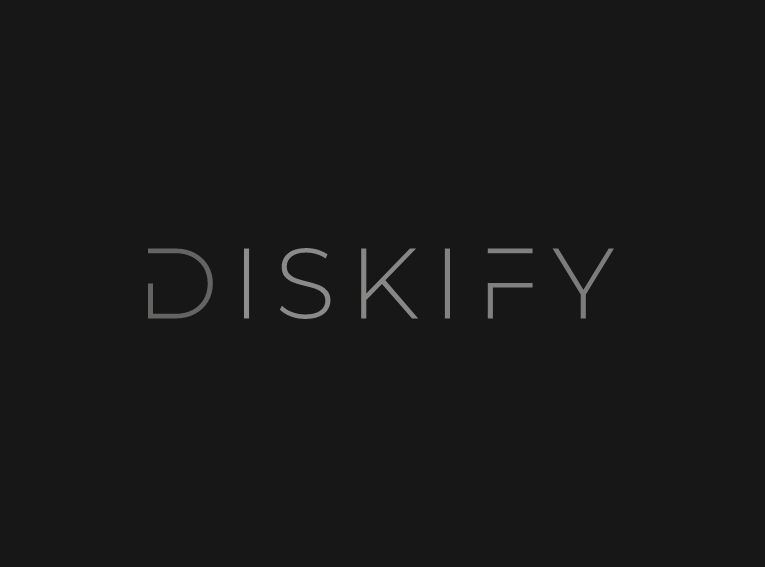
\includegraphics[width=13cm]{ks/diskify.PNG}
    \label{fig:head}
\end{figure}
\FloatBarrier \newpage

$\\ \\ \\ \\ \\ \\$ $\\ \\ \\ \\ \\ \\$ $\\ \\ \\ \\ \\ \\$
\begin{abstract}{\it 
Tokens não-fungíveis (NFTs) se tornaram um atrativo para muitos mercados, um notável caso de sucesso de tecnologia baseada  em blockchain. NFTs são baseadas em contratos inteligentes (Smart Contracts) e são usadas para a definição e transferência de direitos de propriedade, representando vários tipos de dados. O projeto Diskify aproxima a indústria da música de seus fãs, promovendo escassez de conteúdo e eliminando intermediários como aplicativos de streaming e produtoras.
}\end{abstract} \newpage \tableofcontents \newpage

\section{Introdução}

Desde 8 de março de 2020, o mercado de criptomoedas tem crescido e atingido máximas históricas mensalmente (COINMARKETCAP, 2021). A procura por esses tipos de ativos aumentou devido à preocupação de investidores com o futuro da economia em meio à corrente situação pandêmica. Os motivos que os levam a optar por essas moedas são, geralmente, desconfiança do lastro de suas moedas fiat – isso deve-se à quebra do acordo de Bretton Woods em 15 de agosto de 1971: quando o governo do presidente americano, Richard Nixon, encerrou a convertibilidade do dólar em ouro; até antes dessa mudança, um cidadão americano poderia ir ao banco e trocar cada dólar que tivesse por uma quantia em gramas de ouro fixa. Perceba que, a partir deste momento, o dólar se torna uma moeda fiduciária (moeda fiat), uma moeda sem lastro em algum metal precioso, como ouro ou prata, mas com lastro na confiança de seus usuários em quem as emite, bancos centrais em serviço do Estado. Países como Japão, Suíça e Rússia compraram ouro dos Estados Unidos pós o rompimento do sistema de Bretton Woods para ficaram independentes de crises americanas e possuírem reservas de valor próprias. Os eventos ocorridos em 2020 com relação à COVID-19 não possuem precedentes históricos, estamos mais conectados e sintonizados nas notícias sobre o que está acontecendo ao redor do mundo. Como muitas empresas foram fechadas temporariamente e outras para sempre, pessoas ficaram sem empregos e precisavam de subsídios para se manter durante esse período, de janeiro a junho do mesmo ano, mais de 20\% de todo o dinheiro existente em 2019 foi impresso (ROBERTSON, 2020), isso implica em todas as reservas físicas até então se desvalorizando o equivalente em porcentagem; pois imprimir dinheiro não é gerar valor, e inflacionar não equivale em estimular o consumo. Fatos como este impulsionam investidores mais conservadores a buscarem alternativas fora de seu perfil de risco para proteger seu capital, a busca por moedas deflacionárias como o Bitcoin – uma moeda deflacionária é um ativo que tende a se manter em quantidade limitada e escassa, ou seja, a oferta da moeda é fixa e a demanda por ela tende a aumentar com o tempo; no caso do bitcoin, por ser a primeira delas, muitos mineradores armazenaram suas chaves privadas em discos rígidos ou em carteiras aos quais perderam o acesso, portanto, na prática, ainda que o número máximo de bitcoins seja 21 milhões de moedas, há um número menor delas em circulação – o que corrobora com o aspecto deflacionário e a propulsiona em termos de valor de mercado; muitos críticos afirmam que o bitcoin, em especial, é uma pirâmide financeira e que precisa de lastro do Estado para funcionar, porém, não percebem que o lastro do bitcoin remanesce na matemática pois o abastecimento da moeda é fixo e ela mantém os registros das trocas entre usuários na blockchain, evitando que transações falsas sejam realizadas. Afinal, o objetivo de uma moeda é facilitar trocas e manter suas reservas de valor.

\FloatBarrier
\begin{figure}[h]
    \centering
    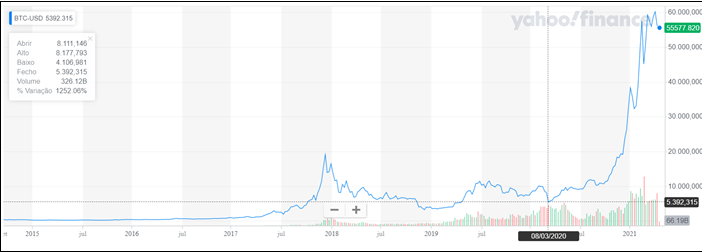
\includegraphics[width=15cm]{fs/f11.PNG}
    \caption{Valorização do Bitcoin entre 04/03/2020 e 20/04/2021.}
    \label{fig:f11}
\end{figure}
\FloatBarrier

Considerando as criptomoedas (descentralizadas) como o futuro da economia, aplicações de finanças decentralizadas (DeFi – decentralized finance) e NFTs (NAPOLETANO, 2021) obtiveram um enfoque da comunidade de investidores cripto, tendo aumentado o seu valor de mercado durante a pandemia também. Elas visam a remover um intermediário de produtos financeiros, tornando o indivíduo em seu próprio banco ou corretora. NFTs, tokens não fungíveis, são colecionáveis com direito de propriedade: o uso deles tem sido adotado por fãs da arte moderna, sendo muitas obras digitais salvas em rede blockchain e suas NFTs negociadas entre usuários. O artista conhecido como Beeple leiloou uma de suas artes digitais por 69 milhões de dólares na casa de leilão Christie’s em 11 de março de 2021 (Figura 1-2), ele está entre os três artistas vivos mais valiosos atualmente. Uma pergunta recorrente é por que alguém compraria uma imagem que pode ser facilmente replicada ou por que alguém pagaria para ter algo que pode ver gratuitamente; a resposta para esse tipo de comportamento é que as pessoas são coletoras, gostam de colecionar objetos mais pelo valor que veem neles do que uma finalidade ou utilidade tão somente, pois o valor de objetos é sempre subjetivo e está fora dele à mercê das trocas voluntárias entre indivíduos; igualando-se aos motivos pelos quais um comprador pagaria preços exorbitantes na Monalisa, mesmo que esta obra seja amplamente conhecida e já replicada, pois cabe aqui a ideia de propriedade sobre o objeto. Com as várias aplicabilidades de um NFT, alguns projetos almejam integrá-las em contratos de propriedade física, como uma rede de NFTs para apartamentos que permita uma troca fácil e direta, outros desafiando os padrões da arte contemporânea.

\FloatBarrier
\begin{figure}[h]
    \centering
    
\includegraphics[width=12cm]{fs/f12.PNG}
    \caption{NFT de Beeple negociada na Christie’s: Everydays – The First 5000 Days.}
    \label{fig:f12}
\end{figure}
\FloatBarrier

Diskify é um projeto que integra a indústria musical à tecnologia das NFTs. Músicos menos populares ficam sujeitos a gravadoras e aos direitos autorais que elas têm sobre suas produções. Com a plataforma proposta, os artistas podem vender álbuns – havendo um limite de cópias definido pelo artista, o que aumenta a raridade do produto –, eliminando a porcentagem da receita líquida que vai para as gravadoras e gerando uma fonte de renda alternativa para que não dependam de seus shows apenas. Como há uma raridade em cada álbum, fãs podem acordar um preço pelo produto de forma subjetiva – pois a plataforma Diskify em muito se assemelha à uma Exchange de valores ou um Marketplace digital – e, se a posteriori decidirem revendê-los, haverá um mecanismo conhecido como royalties utilizado em NFTs de arte digitais: é uma forma de recompensar o artista pelo seu trabalho, a cada troca feita uma porcentagem do preço acordado é repassada ao músico. 

Portanto, o projeto Diskify é uma plataforma de livre acesso e negociação de bens digitais que possibilita trocas de álbuns musicais por criptomoedas, integrando o direito de propriedade sobre o álbum em NFTs e as armazenando em carteiras digitais cripto, se o usuário assim desejar. Com uma NFT, o fã pode baixar para seu dispositivo as músicas e reproduzi-las, mas, caso queira revender seu token, as terá removidas de seu dispositivo. Isso não impede que algum usuário regrave as músicas e as poste em alguma outra plataforma, mas isso configura pirataria e continuará sendo um item de menor valor subjetivo do que o original.

\FloatBarrier
\begin{figure}[h]
    \centering
    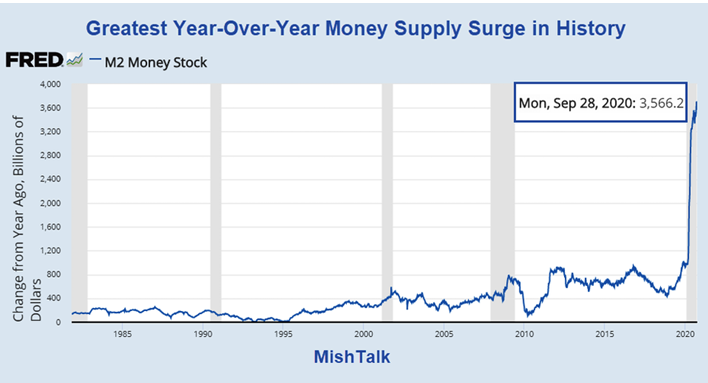
\includegraphics[width=12cm]{fs/f13.PNG}
    \caption{2020, o ano de maior impressão de dólares na história.}
    \label{fig:f13}
\end{figure}
\FloatBarrier

\subsection{Modelo do Plano de Negócios e Personas}

O modelo se segue abaixo:

\FloatBarrier
\begin{figure}[h]
    \centering
    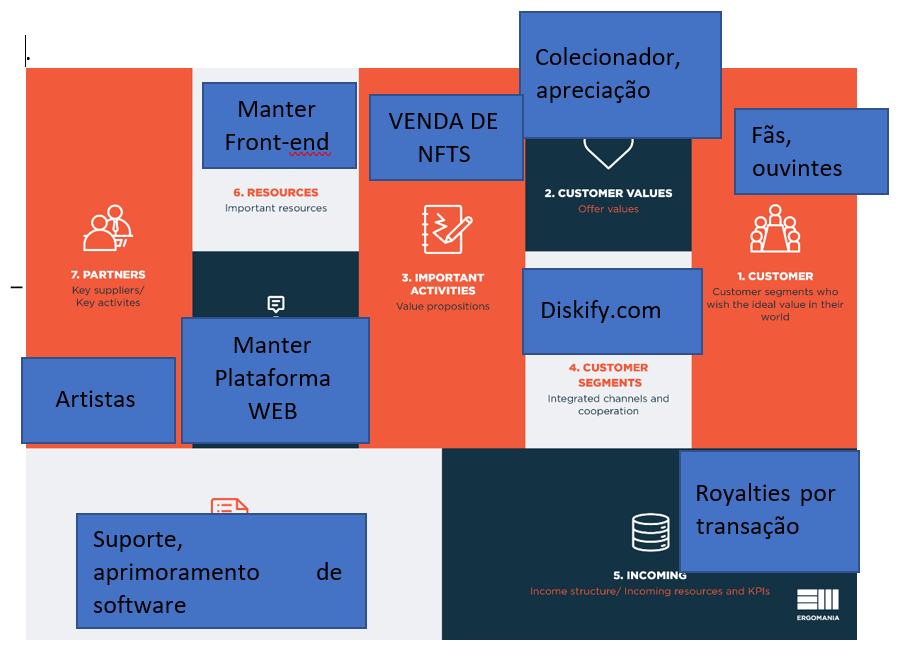
\includegraphics[width=12cm]{fs/BMC.PNG}
    \caption{Business Model Canvas.}
    \label{fig:bmc}
\end{figure}
\FloatBarrier

Como a empresa pretende mitigar custos e gerar inovação:

\FloatBarrier
\begin{figure}[h]
    \centering
    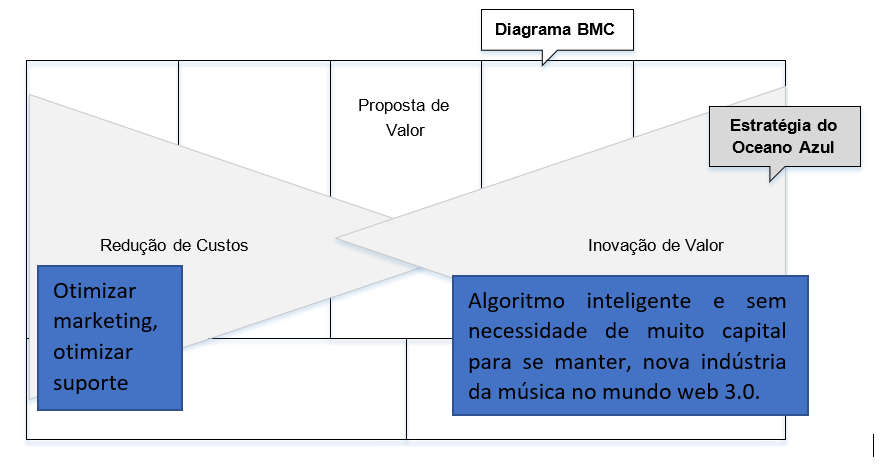
\includegraphics[width=12cm]{fs/bmc2.PNG}
    \caption{Soluções: mitigação de custo.}
    \label{fig:bmc2}
\end{figure}
\FloatBarrier

Questões-chave sobre o nosso modelo:

\FloatBarrier
\begin{figure}[h]
    \centering
    
\includegraphics[width=12cm]{fs/g1.PNG}
    \caption{Questões-chave: parte 1.}
    \label{fig:qc1}
\end{figure}
\FloatBarrier

\FloatBarrier
\begin{figure}[h]
    \centering
    
\includegraphics[width=12cm]{fs/g2.PNG}
    \caption{Questões-chave: parte 2.}
    \label{fig:qc2}
\end{figure}
\FloatBarrier

\FloatBarrier
\begin{figure}[h]
    \centering
    
\includegraphics[width=12cm]{fs/g3.PNG}
    \caption{Questões-chave: parte 3.}
    \label{fig:qc3}
\end{figure}
\FloatBarrier

Matriz de Inovação de Valor:

\FloatBarrier
\begin{figure}[h]
    \centering
    
\includegraphics[width=12cm]{fs/h1.PNG}
    \caption{Matriz de inovação de valor.}
    \label{fig:h1}
\end{figure}
\FloatBarrier

Personas:

\FloatBarrier
\begin{figure}[h]
    \centering
    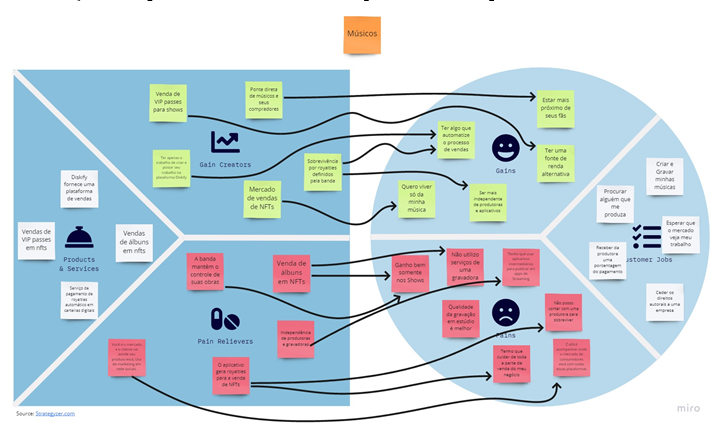
\includegraphics[width=12cm]{fs/pers1.PNG}
    \caption{Modelo para o Canvas da Proposta de Valor para Músicos. Fonte: Strategyzer.}
    \label{fig:p1}
\end{figure}
\FloatBarrier

\FloatBarrier
\begin{figure}[h]
    \centering
    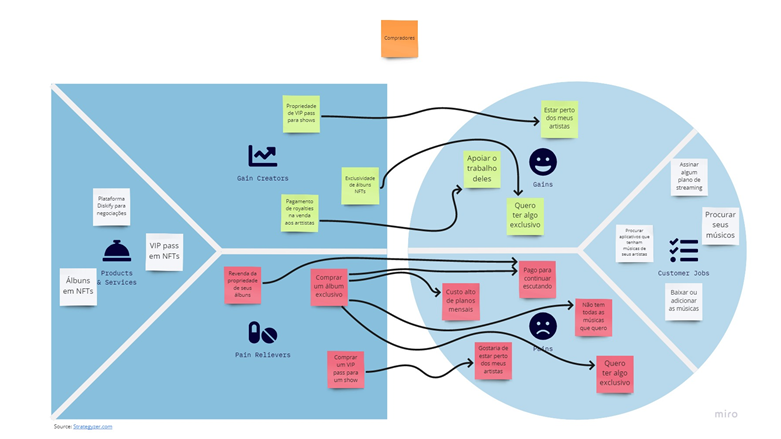
\includegraphics[width=12cm]{fs/pers2.PNG}
    \caption{Modelo para o Canvas da Proposta de Valor para Consumidores. Fonte: Strategyzer.}
    \label{fig:p2}
\end{figure}
\FloatBarrier

\section{Análise Ambiental}

As empresas são sistemas abertos influenciadas pelo mercado no qual estão
inseridas. Nesta seção, será abordado o ambiente externo e interno da empresa {\it Diskify}.

\subsection{Macro-Ambiente}
\iffalse (Político-Legal; Econômico; Sócio-Cultural; Tecnológico) \fi

Para discorrer sobre esses aspectos, será ressaltada a visão política da administração da empresa - sim, estamos cientes das implicações resultantes do nosso posicionamento; para isso, desenvolvemos soluções para evitar os pontos a seguir.

No que tange ao aspecto Político-Legal, somos altamente libertários segundo quadrante político\cite{espp}; observe que todo nosso modelo de negócios se dá através de redes de dinheiro em blockchain descentralizadas. Estamos cientes de que, enquanto empresa, seria necessário uma burocracia para com nós dependendo do país em que a empresa estiver localizada. Porém, tomamos em consideração que, para que nosso modelo seja o mais custo-oportunidade para ambas as personas da plataforma, deveremos manter toda a parte de taxação fora do mecanismo de distribuição de royalties em vendas criados por nós. Para isto, a empresa terá sua parte de cada transação anonima definida pelo músico e será efetuada a cada movimentação na rede e depositada na carteira virtual da empresa - esta pode até vir a ser rastreada para fins de transparência com as autoridades, mas pensando em aumentar os lucros e evitar leis "anti-performistas" de certos países, a empresa está negociando a possibilidade de criar a sua central (header administrativo) em algum país do Caribe, Estônia, Malta ou Portugal, pois estes possuem uma política de lucros e taxação com as quais a empresa simpatiza \cite{crpt} (veja esta citação para mais informações da empresa parceira nesta parte de localização e taxação).

No que tange ao aspecto Econômico, estamos voltados para o desenvolvimento do mundo DeFi nas finanças modernas atuais - como entusiastas, gostamos da ideia de que cada pessoa pode eliminar o "player" banco de suas equações no dia a dia e que pode utilizar de artifícios complexos para suas negociações interpessoais sem nenhum acréscimo de terceiros. Para este aspecto, levamos em conta o crescimento de bilhões investidos neste mercado e avaliamos como uma tendência futura (expectativa de maturação entre 3 a 5 anos)\cite{defi}. Toda a movimentação com relação ao capital das personas envolvidas diz respeito a elas e seus patrimônios de forma que a empresa não se interessa muito com que forma eles foram obtidos. Mas, como ressaltado nas seções acima, o público inicial desse projeto é investidor e especulativo primariamente e um subgrupo de entusiastas ou fãs de música, o que nos habilita a esses pensamentos: 1) o PIB de seus países em nada influência o consumo destes pelos nossos produtos: são consumidores de classe A, B e C - pois todos na rede atualmente têm capital para especular; 2) a disponibilidade e o custo de energia é praticamente nulo para as personas e, para a empresa, baixo; 3) quanto maior a inflação de moedas FIAT, melhor para o mercado cripto e melhor para a empresa por conseguinte; 4) o crescimento econômico é irrelevante para o mercado cripto pois o capital já é escoado para este mercado em tempos ruins e, em melhores, ainda mais; 5) quanto maior a tributação de outros sobre serviços de streaming e similares, melhor, pois isso favorece a nós intolerantes a esse abuso; 6) com respeito a juros, em nada nos afeta - nem o juros de longo prazo (TJLP, 7).

No que tange ao aspecto Sócio-Cultural, a nossa empresa nada mais é que o meio da web 3.0 para propagar essas mudanças com os nossos produtos - porém, não devemos, em respeito aos artistas, fazer julgo das implicações de suas obras, pois vemos todas como Arte apenas e não finalidades para incitar agressões ou quebras ao PNA (pacto de não-agressão, única cartilha que seguimos de fato, fora os postulados de Hans-Hermann Hoppe sobre propriedade e individualidade). Em suma, se alguma música for de caráter ofensivo a algum usuário na rede, nada será feito porque somos absolutistas da liberdade de expressão. Algo será feito, no entanto, caso haja a implicação de copyright de alguma de nossas obras.

No que tange ao aspecto Tecnológico, a nossa empresa está na ponta da lança com respeito ao futuro desta indústria que há muito não mais vê grandes atualizações na forma com que as negociações são feitas. Desenvolvemos tanto a tecnologia para negociar os produtos como o formato de novos produtos com os quais os artistas se submeteram para manter suas obras atualizadas na rede; de certa forma, todo o mecanismo é feito para que haja um constante aprimoramento da tecnologia sem que isso custe as personas. Há, também, a possibilidade de a empresa disponibilizar interfaces open-source para que os usuários personalizem o aplicativo e decidam qual usar; é do nosso interesse que o smart contract desenvolvido seja altamente integrável.

\subsection{Ambiente Setorial}
\iffalse (Forças de Porter; Stakeholders) \fi

Sobre o nosso ambiente setorial, nos vemos como uma empresa muito plástica ainda, pois possibilitamos o caráter anti-corporativo para nosso modelo empresarial - isso implica que nossos stakeholders: 1) consumidores, são os que mais atuam sobre o algoritmo e definem o valor de todos os colecionáveis transacionados, como definimos um mecanismo de preço flutuante, o preço destes itens é definido em consenso pelo subjetivismo coletivo dos compradores (logo, cada colecionável se comporta como uma commoditie que pode ser ou não apreciada com o tempo); 2) as empresas concorrentes têm o comportamento de clubismo entre os integrantes músicos de suas plataformas ao passo que nós permitimos a qualquer endereço na rede se tornar um membro produtor da plataforma e não apenas ouvinte (criamos mecanismos anti-span para auxiliar na mitigação da infração de copyright); 3) os fornecedores são os músicos no nosso cenário, damos a eles máxima liberdade para definir o mecanismo de royalties e como serão pagos pelas suas obras quando estas forem transacionadas; 4) somos anti-sindicatos e, possivelmente, uma das primeiras empresas a acabar com esta vergonha moderna - cada músico é seu próprio empresário para fins técnicos (já que estes se importam tanto com o rigor técnico de seus rabiscos infundados que ousam afirmar lei), estaremos nos movendo para offshores como apontado e o caráter de comunicação, transação e afins da empresa estará declarado na própria blockchain com seus registros de cada ação efetivada na plataforma, não existirá um sequer endereço na rede - que utilize os nossos serviços - prejudicado por nós ou por outros endereços na rede pois tudo estará descrito nos nossos termos de serviço e, para explicitar um caso onde haja a infração de copyright de outrem, a empresa manterá o capital travado das obras negociadas durante o prazo estipulado de 1 mês para ressarcir usuários prejudicados e parte dos royalties obtidos da empresa será utilizado para esse fim caso algo do tipo ocorra; 5) não haverá acionistas iniciais desta empresa fora os proprietários aqui neste trabalho citados, sim, a possibilidade de mais acionistas adentrarem a empresa se dará de forma "não-legal", pois faremos um mecanismo na blockchain de divisão dos fundos no endereço do smart contract do aplicativo da empresa, esse endereço redirecionará os fundos as carteiras que possuírem os tokens da empresa (acionistas, que podem ser quaisquer usuários na rede que tiverem nosso token de empresa) percentualmente; 6) o setor financeiro de nossa empresa não existe a priori, pois não precisamos de contadores e especialistas desse tipo (pelo menos em demasiado excesso como se vê em outras empresas), quero dizer que os nossos contadores e personel de marketing terá a verba percentual mensal definida para realizar as tarefas almejadas pela a empresa em divulgação e para manter-se em acordo com as autoridades locais da nossa central header definida na seção anterior; e 7) a sociedade pode até esperar coisas de nossa empresa que não faremos e temos dito incansavelmente nos nossos termos, nosso papel será o mesmo desde o início: somos o marketplace de música na web 3.0 e não compactuamos com ideais globalistas nos nossos atos para com os nossos artistas em questão de julgo.

Para definir as Forças de Porter a seguir, reforçamos que chegar as estas conclusões foi um trabalho de muito tempo e quebra de paradigmas de pensamento sobre vendas. Somos uma empresa que foca no anti-frágil, perceba que, se um disco é vendido por X, não temos nada a ver com o vendedor e comprador nessa transação (fora todo o caráter tecnológico de nossa parte e de sermos a ponte para isso) e que esta obra é uma NFT, então, não pode ser comercializada em outro lugar que não no nosso pois é uma transação de caráter singular - só pode existir aqui e agora -; no entanto, NFTs de áudio podem ser desenvolvidas por outros aplicativos na rede e também podem ser negociadas por nós na nossa plataforma; a empresa logo atua como a garantia não só de ser um novo marketplace para os músicos, bandas, artistas etc., como também fornece os serviços de copyright a estes (sendo então a primeira a fornecer copyright para esse tipo de produto na web 3.0.) e é uma alternativa ao modelo de streaming atual de empresas do mundo web 2.0, como {\it Spotify}. A ameaça de novos entrantes é baixa, pois somos toda a rede em caráter de negociação e, dificilmente, o músico estaria interessado em estar no {\it Deezer} e {\it Spotify} da web 3.0 porque essa é a visão errada da abordagem (a plataforma do usuário pode ser qualquer, a roupagem do algoritmo não nos interessa - estaríamos tranquilos caso uma empresa se especializasse em ser nosso front-end; não que nós não tenhamos o nosso, temos, é que se isso ocorresse, haveria taxas adicionais, o que dificulta o surgimento de concorrentes para o nosso modelo). O poder de negociação de nossos consumidores não é tão relevante porque, caso percam ou ganhem, haverá mercado crescente ainda sim, pois somos um serviço de luxo (o caráter da empresa se dá pela necessidade de ser um colecionador e ter algo que é escasso, o interesse por coisas do tipo nunca acaba, a riqueza e estes artigos são apenas transferidos). Os fornecedores não são contra nós e não podem ser, são eles que definem o preço justo pelas suas obras seus royalties e o quanto nós ganharemos pelo serviço a eles fornecido; se o artista definir que ganha 1\% de royalties sobre transações feitas com seu material, a empresa também ganhará 1\% - e isto está definido nos nossos termos de negócio. A ameaça de produtos substitutos é a mais alta delas, pois novos estilos de produtos podem surgir, para isso, definimos um token padrão que servirá para todas as negociações independente do produto comercializado (pode ser um vídeo ou algum ingresso para show, e não um álbum de músicas necessariamente), esta ameaça se tornará maior com a expansão do mercado, mas o cuidado com novas tendências na indústria nos dá vantagem para atualizar nossos serviços.

Note que descrevemos que novos entrantes, no esquema de Forças de Porter, não são um problema para nosso mercado porque somos altamente flexíveis ao conteúdo que eles poderiam comercializar, na verdade, eles nos ajudariam e não teriam espaço sem muito investimento em suas plataformas até que pudéssemos concorrer igualmente; neste tempo, a {\it Diskify} já teria o tamanho para ser o principal serviço deste tópico na web 3.0. Mas note, também, que não acreditamos em concorrência interna atualmente pois sabemos que todas os aplicativos semelhantes ao nosso modelo de negócios ou são limitados em cobertura de atividades na indústria da música (às vezes, só criam NFTs, outros estão lá só para vender tokens da empresa, a ideia dela ainda, em vez de bons produtos), ou estão em outras blockchains - e este, talvez, seja nosso maior ponto positivo com relação ao mercado, pois estamos dentro da rede Ethereum - a maior rede de soluções em 2a camada e a mais antiga também, o que implica mais investidores e mais capital; alguns especialistas dizem que é a rede mais valiosa dentre as redes de smart contracts de 2a ou 3a geração por já ter aplicabilidades hoje -, nossos concorrentes se encontram em redes como Solana, Avalanche etc.: redes que têm poucos aderentes e, certamente, mais instabilidades e insegurança.
 
\subsubsection{Mais Sobre as Forças de Porter}

A força 1, possibilidade de entrada de concorrentes, teve uma média de 2.1, o que caracteriza como força média.

A força 2, rivalidade entre as empresas do ramo, teve uma média de 2.0, há média rivalidade entre concorrentes.

A força 3, ameaça de produtos substitutos, teve uma média de 3.75, há alta ameaça de produtos substitutos.

A força 4, poder de negociação dos compradores, teve uma média de 2.5, há médio poder de compra dos clientes.

A força 5, poder de negociação dos fornecedores, teve uma média de 1.6, demonstra que os fornecedores afetam em menor grau o setor.

A média geral do setor é de 2.39, a empresa está situada em um ambiente de intensidade competitiva média, a empresa deve-se atentar a uma boa comunicação com os seus compradores, e buscar desenvolver novos produtos para manter-se competitiva no mercado.

\subsection{Oportunidades e Ameaça}

Como citado nas seções anteriores, poucos projetos têm um oceano azul tão azul quanto o nosso; é um fenômeno raro de se observar. As oportunidades estão em excesso neste meio e há poucas ameaças, porém, severas. Vamos listar as 3 melhores oportunidades segundo à nossa visão: 1) a rede Ethereum carece de um aplicativo que permeie todo esse espectro desenvolvido até aqui sobre nossos meios de atuação (ver seção anterior); 2) queremos ressuscitar um comportamento morto nos anos 90 sobre a noção de se ter coisas exclusivas ou raras e, de fato, possuí-las, sem ter que pagar mensalidades para sempre para escutar as mesmas músicas; e 3) estamos pensando em sermos um novo modelo de copyright e organizadores de ingressos de eventos, principalmente, musicais - facilitando o processo de entrar em shows e/ou comprar ingressos vip (isso é um mercado que pode ser explorado até pós o show, há a história de ingressos do lollapalooza que foram revendidos na Ebay para colecionadores - de novo a ideia de itens colecionáveis raros gerando royalties). Sobre as ameaças, 3 delas: 1) pouco público no início, baixo retorno - é um meio inundado por investidores majoritariamente e poucos consumidores, muitos fãs não entendem muito de economia, lógica de preços, oferta e demanda ou blockchains e NFTs -, isso tudo, no entanto, é temporário e já está adentrando o imaginário de jovens; 2) suporte aos músicos, muitos músicos não têm facilidade com tecnologia, talvez apenas as de mixagem de som, o suporte da nossa empresa seria de caráter educativo com vídeos e explicações no nosso site sobre como atuamos ou contatos de membros da comunidade para esclarecimentos de dúvidas; e 3) a indústria antiga poderia atacar o nosso modelo disruptivo por não compactuar com a nossa de remoção deles do fluxo de negócios, pois destruiremos o modelo deles, para isso, estaremos localizados em safe-havens comerciais e burocráticos e nosso serviço não poderá ser removido ou banido porque estaremos na web descentralizada. 

\subsection{Ambiente Interno}
\iffalse (Infraestrutura; Gestão; Marketing; Produção/Operações; Pessoas – RH; Finanças) \fi

Nesta seção, destacaremos nossa condutas com relação aos tópicos do ambiente interno da empresa. Os nossos pontos positivos e negativos foram elicitados na seção anterior e serão compreendidos de forma descritiva aqui.

Planejamento: será realizado por nós e se dará com relação aos modelos de produtos comercializados, gestão de royalties, marketing e divulgação para novos músicos. Ponto forte: estamos atuando de forma otimizada.

Gestão: executará o planejamento acima e cuidará das pendências da empresa, será feita pelos encarregados da proposta. Ponto forte: equipe limitada e eficiente atuando em um mercado sem regulações.

Sistema de Informações: será desenvolvido pela empresa e seus programadores e compreenderá todas as necessidades tecnológicas da empresa. Ponto forte: nossa tecnologia é a mais nova e feita para se ajustar com o que queremos exatamente.

Infra-estrutura: irrelevante, a estrutura já existe e pertence às blockchains, teremos um repositório que renderizará o front-end reativo da aplicação e o número de requisições simultâneas será equilibrado com load-balancing de provedores terceirizados. Ponto forte: já está pronta e tem baixo custo.

Mercadológicos: faremos uso total de marketing holístico e algumas propagandas custeadas com os royalties obtidos pelo o aplicativo e venda das shares da empresa em forma de tokens. Ponto fraco: não queremos despender capital demais com esta área, mas será mais necessário com a expansão da empresa.

Pessoas: precisaremos de uma pequena equipe para desenvolver a política de vendas e suporte, toda ela será mantida com o capital de giro da empresa. Ponto forte: nossa equipe é facilmente conduzida a atuar em problemas novos de caráter prático-social, pouco teor tecnológico envolvido.

Operação: o custo dela será baixo comparado a outros serviços de streaming, o nosso custo deve ser pago com transações recorrentes de nossos produtos. Ponto forte: nossa equipe pode atuar com pouco e ser lucrativa pois não depende de estruturas complexas para resolver a nossa lógica de negócio.

Finanças: são feitas com o nosso modelo on-chain de contabilidade através do framework moralis com os mecanismos de transações desenvolvidos por nós. Ponto forte: resolvemos tudo por algoritmos e está tudo em framework virtualizador de blockchains customizável para fins de demonstração de conteúdo.

Relacionamento com a sociedade: temos um posicionamento neutro, essa é a política. Ponto forte: estamos por nós e a comunidade sempre.

\subsection{Forças e Fraquezas}

Descrevemos os nossos pontos de atuação nas duas seções anteriores e discorremos sobre o embate deles contra nossos competidores nesta. Nossos competidores mais relevantes são BlueBox e Audius. Nossos fatores críticos de sucesso são bem simples: precisamos manter o acesso à nossa plataforma o mais aberto possível e evitando o clubismo de músicos que ambas competidoras pregam a escolher e definir apenas "artistas confiáveis" - ou melhor, aqueles que compactuam ideologicamente, ou porque elas são empresas desse caráter, ou porque não têm mecanismos anti-span como a nossa empresa, que os desenvolveu em smart contracts -; apenas isso aliado do fator de estarmos na maior rede, Ethereum, é o suficiente para termos a maior fatia do mercado.

Avaliação das nossas forças e fraquezas se dará por avaliar os pontos da seção anterior, pois descrevemos tudo conectadamente nas seções 2.3, 2.4 e 2.5. Nosso planejamento é o mais expansivo dentre as 3 empresas (Diskify, Audius e BlueBox); temos a melhor gestão, sistema de informações, infra-estrutura, operação, finanças, pessoas (equipe)  e relacionamento com a sociedade que as demais; nossas práticas de marketing são as menos avançadas dentro do cenário no entanto.

Com relação à indústria, todos os pontos são fortes pois somos bem disruptivos, mas - para elencar - as 3 principais seriam planejamento, finanças e infra-estrutura.

\subsection{Matriz SWOT - Matriz de Avaliação Estratégica}

Nesta seção, mostramos a matriz SWOT, sua legenda e seu PEG. Atente-se aos nomes dados às oportunidades, ameaças, forças e fraquezas: foram discorridos nas seções acima.

\FloatBarrier
\begin{sidewaysfigure}[h]
    \centering
    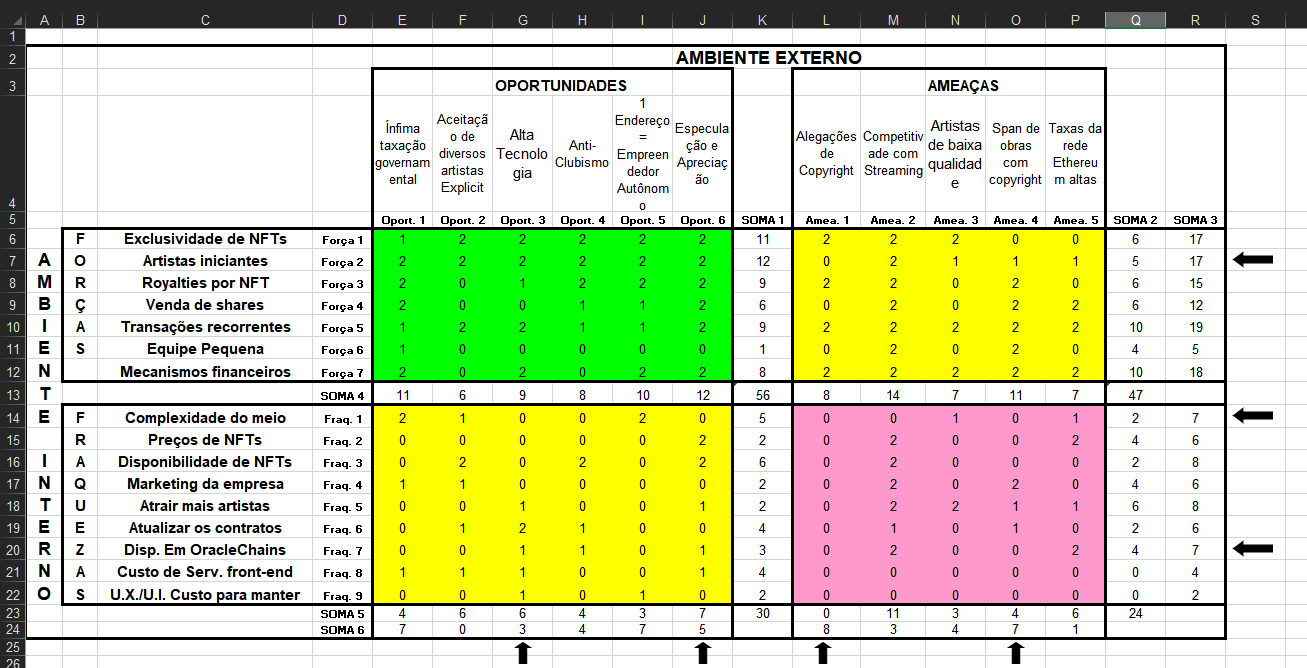
\includegraphics[width=25cm]{gs/mgeral.PNG}
    \caption{Matriz SWOT.}
    \label{fig:gs1}
\end{sidewaysfigure}
\FloatBarrier

\FloatBarrier
\begin{sidewaysfigure}[h]
    \centering
    
\includegraphics[width=25cm]{gs/description.PNG}
    \caption{Legenda.}
    \label{fig:gs2}
\end{sidewaysfigure}
\FloatBarrier

\FloatBarrier
\begin{figure}[h]
    \centering
    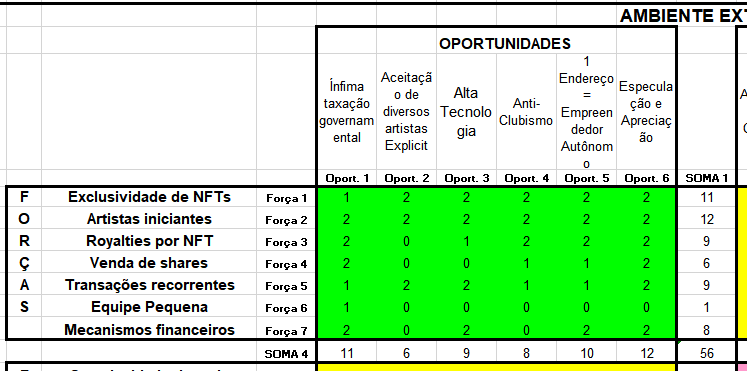
\includegraphics[width=12cm]{gs/quad1.PNG}
    \caption{Quadrante 1.}
    \label{fig:gs3}
\end{figure}
\FloatBarrier

\FloatBarrier
\begin{figure}[h]
    \centering
    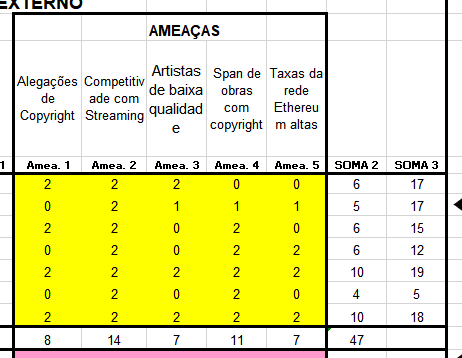
\includegraphics[width=12cm]{gs/quad2.PNG}
    \caption{Quadrante 2.}
    \label{fig:gs4}
\end{figure}
\FloatBarrier

\FloatBarrier
\begin{figure}[h]
    \centering
    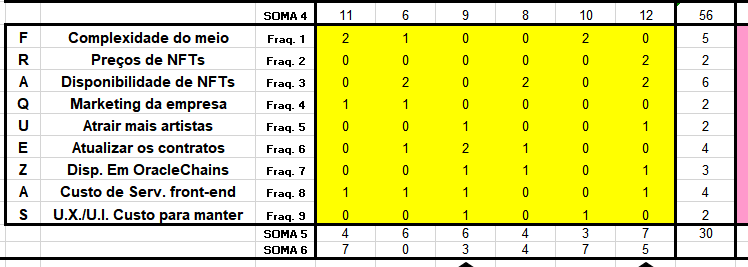
\includegraphics[width=12cm]{gs/quad3.PNG}
    \caption{Quadrante 3.}
    \label{fig:gs5}
\end{figure}
\FloatBarrier

\FloatBarrier
\begin{figure}[h]
    \centering
    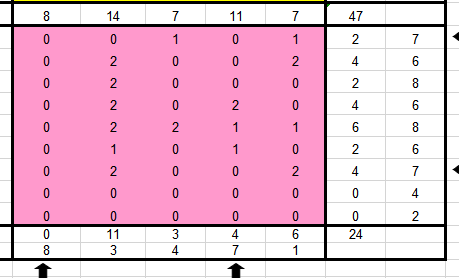
\includegraphics[width=12cm]{gs/quad4.PNG}
    \caption{Quadrante 4.}
    \label{fig:gs6}
\end{figure}
\FloatBarrier

\FloatBarrier
\begin{figure}[h]
    \centering
    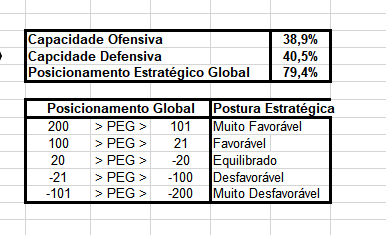
\includegraphics[width=12cm]{gs/peg.PNG}
    \caption{Posicionamento estratégico Global.}
    \label{fig:gs7}
\end{figure}
\FloatBarrier

\section{Formulação Estratégica}
\iffalse (Missão; Visão; Objetivos Estratégicos e Estratégias) \fi 

Nesta seção, abordamos o ideal da empresa e suas condutas.

\subsection{Missão}

A razão de ser da {\it Diskify} tem como objetivo a criação de um Marketplace de negociação de NFTs de álbuns musicais, a facilitação para músicos de venderem suas obras de forma independente de produtoras e a criação de uma fonte alternativa de renda.  

O público-alvo do projeto Diskify se divide em duas personas: Músico e Comprador. Músico é todo aquele indivíduo que se interessa por publicar seus trabalhos artísticos e musicais na plataforma de forma a automatizar o processo de vendas e pagamento de royalties. Comprador é todo fã interessado em consumir algum álbum produzido por artistas. As entrevistas feitas limitaram-se aos dois perfis e às suas dores. Nossas personas e seu comportamento no canvas de proposta de valor foram figurados na seção 1.1.

A descrição de negócio da Diskify é um projeto que integra a indústria musical à tecnologia das NFTs. Músicos menos populares ficam sujeitos a gravadoras e aos direitos autorais que elas têm sobre suas produções. Com a plataforma proposta, os artistas podem vender álbuns – havendo um limite de cópias definido pelo artista, o que aumenta a raridade do produto –, eliminando a porcentagem da receita líquida que vai para as gravadoras e gerando uma fonte de renda alternativa para que não dependam de seus shows apenas. Como há uma raridade em cada álbum, fãs podem acordar um preço pelo produto de forma subjetiva – pois a plataforma Diskify em muito se assemelha à uma Exchange de valores ou um Marketplace digital – e, se a posteriori decidirem revendê-los, haverá um mecanismo conhecido como royalties utilizado em NFTs de arte digitais: é uma forma de recompensar o artista pelo seu trabalho, a cada troca feita uma porcentagem do preço acordado é repassada ao músico. Portanto, o projeto Diskify é uma plataforma de livre acesso e negociação de bens digitais que possibilita trocas de álbuns musicais por criptomoedas, integrando o direito de propriedade sobre o álbum em NFTs e as armazenando em carteiras digitais cripto, se o usuário assim desejar. Com uma NFT, o fã pode baixar para seu dispositivo as músicas e reproduzi-las, mas, caso queira revender seu token, as terá removidas de seu dispositivo. Isso não impede que algum usuário regrave as músicas e as poste em alguma outra plataforma, mas isso configura pirataria e continuará sendo um item de menor valor subjetivo do que o original. 

Um ponto desprezado por produtores e gravadoras: a independência e vontade dos músicos em se autoproduzir e gerar renda, sem abusos de receita ou cláusulas de contrato leoninas; e, também, a desassociação da ideia de que uma empresa detém os direitos de propriedade intelectual sobre sua arte: também, dessa forma, aproximando o consumidor de seus artistas com a possibilidade de deter a propriedade de conteúdos exclusivos. As entrevistas levantaram pontos esperados e ajudaram a estipular que pessoas interessadas em apoiar algum artista também estão dispostas a comprar colecionáveis. Durante as entrevistas, um novo canal de renda para a plataforma Diskify veio à tona, segundo à perspectiva da equipe, seria interessante adicionar a ideia de passes VIP para shows como NFTs para venda na plataforma. Os passes seriam emitidos pelos artistas, tendo a distinção de passes vitalícios que permitiriam aos seus donos de participaram de backstages (espaço ao lado ou atrás do palco em que fãs ou ajudantes ficam durante os shows), e, se não conseguissem participar de algum evento, poderia alugar ou revender o seu passe – sempre, nessas negociações, realizando royalties para os artistas e uma porcentagem ao projeto Diskify. O entrevistado 7 disse não gostar de ter que fazer todo o processo de venda de seus álbuns e arrecadação, abordando a exata intenção do projeto; enquanto isso, o entrevistado 1 disse que gostaria de ter uma fonte de renda com NFTs. Ter a visão dos músicos entrevistados ajudou a adicionar termos e compreender dinâmicas de mercado e subsistência pelas as quais eles se conformam, e como criar um modelo de negócio disruptivo – a Diskify. O projeto Diskify evita ser um impasse na comunicação entre as personas citadas, isso significa que nossa prioridade se dá na garantia da propriedade intelectual das obras. Uma vez que o álbum esteja disponível à venda, a empresa só terá acesso à NFT dele para fins de checagem ao direito de propriedade intelectual.

As condições de desempenho consideradas essenciais para o projeto são, já que o propósito da empresa é remover os {\it middlemen} (intermediários) que existem entre músicos e seus fãs no que tange a distribuição de suas músicas e propriedade intelectual das obras, adotamos, como filosofia da empresa, a ética libertária de conduta dos indivíduos e a sua auto-soberania como prioridades no desenvolvimento do projeto. Afinal, a empresa precisa ser um marketplace auto-sustentável e descentralizado. Logo, a empresa focará em sempre se manter como contra-parte das relações músicos-fãs e evitará intervir nelas, somente quando houver o descumprimento das políticas de termos de serviços da nossa empresa.

\subsection{Visão}

A nossa visão, enquanto empresa, é bastante reducionista e performática com relação à indústria musical: nossa direção é sermos o marketplace de maior renome na web 3.0 quando o assunto for áudio e similares; nossas descobertas tangem o constante expansionismo do mundo do áudio, como melhoras do produto, do conteúdo, mas, também, o mundo periférico a música, como shows e eventos com passes VIPs e acessos aos backstages; e o nosso destino é consolidar a estrutura da empresa no mundo 3.0 ao passe que reformular processos ultrapassados da indústria, atingindo, então, a nossa ambição de sermos o lugar que os usuários vão para apreciar esta arte.

\subsection{Objetivos Estratégicos}

Sobre as nossas opções estratégicas: temos como grande rumo uma intenção e direcionamento forte e único para a organização, concentramos nossos recursos em um único alvo; nossa postura condiz com o nosso posicionamento estratégico global, predominantemente ofensiva, visando melhorar a posição atual de nossa organização no mercado, portanto, utilizaremos ataques em círculos para desmoralizar diversas posições mal defendidas de nossos concorrentes simultaneamente; nosso vetor de negócios se especifica na atuação e core-business (único negócio) com foco em crescimento; e nossa estratégia competitiva se dá por liderança por diferenciação. Nossos objetivos com relação ao ambiente externo são: 1) posição competitiva; e 2) desenvolvimento da linha de produtos ou serviços. Com relação ao ambiente interno, são eles: 1) liderança tecnológica; e 2) eficiência e eficácia. Ressaltamos que esses objetivos têm como foco aumentar nossas forças e alcançar as oportunidades definidas na matriz SWOT na seção 2.6.

\subsection{Estratégias}

Nossas estratégias condizem com o que o projeto precisar manter em foco para crescer no mercado e se aproximar de seu objetivo, melhorando o uso de ativo fixo e novo conforme crescemos ao passo que reduzimos nossos custos aumentando os níveis de automação; e melhorando a comunicação com nossos clientes, também reforçando o marketing da empresa e propulsionando alguns artistas em destaques nas nossas campanhas.

\section{Marketing}

Nesta seção, descrevemos os planos de desenvolvimento, produção e comercialização dos produtos da {\it Diskify}. Avaliaremos as necessidades e os desejos dos nossos prováveis consumidores, focando em dar significado às suas compras e torná-lo parte importante das mecânicas comerciais da empresa com base nas suas satisfações sobre nossos produtos.

\subsection{Descrição do Negócio}

O projeto Diskify tem como objetivo a criação de um Marketplace de negociação de NFTs de álbuns musicais, a facilitação para músicos de venderem suas obras de forma independente de produtoras e a criação de uma fonte alternativa de renda.

Diskify é um projeto que integra a indústria musical à tecnologia das NFTs. Músicos menos populares ficam sujeitos a gravadoras e aos direitos autorais que elas têm sobre suas produções. Com a plataforma proposta, os artistas podem vender álbuns – havendo um limite de cópias definido pelo artista, o que aumenta a raridade do produto –, eliminando a porcentagem da receita líquida que vai para as gravadoras e gerando uma fonte de renda alternativa para que não dependam de seus shows apenas. Como há uma raridade em cada álbum, fãs podem acordar um preço pelo produto de forma subjetiva – pois a plataforma Diskify em muito se assemelha à uma Exchange de valores ou um Marketplace digital – e, se a posteriori decidirem revendê-los, haverá um mecanismo conhecido como royalties utilizado em NFTs de arte digitais: é uma forma de recompensar o artista pelo seu trabalho, a cada troca feita uma porcentagem do preço acordado é repassada ao músico.

Portanto, o projeto Diskify é uma plataforma de livre acesso e negociação de bens digitais que possibilita trocas de álbuns musicais por criptomoedas, integrando o direito de propriedade sobre o álbum em NFTs e as armazenando em carteiras digitais cripto, se o usuário assim desejar. Com uma NFT, o fã pode baixar para seu dispositivo as músicas e reproduzi-las, mas, caso queira revender seu token, as terá removidas de seu dispositivo. Isso não impede que algum usuário regrave as músicas e as poste em alguma outra plataforma, mas isso configura pirataria e continuará sendo um item de menor valor subjetivo do que o original.

\subsection{Análise da Concorrência}

Diskify não possuí concorrentes diretos no que tange o ideal total do projeto, pois as duas concorrentes, no mundo web 3.0, Audius e BlueBox, se encontram nas blockchains concorrentes - e já bastante conhecidas pelo público-investidor que deve se manter um certo cuidado com elas - binance smartchain e solana; devido a problemas com o Proof-Of-Stake ou volatilidade no preço, manter ativos NFTs com o viés que temos nessas redes seria difícil e não-atrativo, há também um adicional a tudo isso: muitos projetos de NFTs movem-se para redes secundárias com a desculpa de ser de 3a e mais apta ao projeto, no entanto, sofrem desses problemas e falta de maturação - mas, também, muitas dessas empresas alegam que suas práticas se tornariam impossíveis na primeira, maior e melhor rede blockchain inteligente, Ethereum, algo que o nosso projeto resolveu e tornou viável, junto do nosso modelo de distribuição dos dados de transação, mecanismo de royalties e armazenamento de conteúdo atrelado ao NFT; tudo sem aumentar o custo da transação, do mint ou de gas fees. 

Essas duas empresas se encaixam, portanto, junto dos nossos concorrentes indiretos, que são a web 2.0 no geral: Spotify, Deezer, Youtube Music (entre outros não relevantes). Elicitaremos seus pontos fracos a seguir: 1) todos esses serviços são por assinatura, tirando a Audius e a BlueBox que ainda não têm mercado ativo e podem ser desprezados nesse ponto; 2) há um constante reajuste de mensalidades e muitos planos, o que torna tudo mais complexo, mas também possibilita que haja sempre um aumento geral dos preços dessas plataformas por questões de serviços e taxações nos países em que a compra é feita; 3) há um completo descaso com usuários interessados em apenas escutar as 10 músicas de sempre, todos eles relevam o fato de você não consumir nada de novo e o cobram para escutar o que já escutava, em outras palavras, você não é dono e não pode fazer o que quiser com o que é seu; 4) há a possibilidade de mudança de políticas dessas empresas para agradar o status quo e a massa, seu artista fez uma crítica? Poxa, você não pode escutá-lo mais porque a manada está revoltada com ele: isso não acontece com conteúdo descentralizado e registrado em blockchains - uma vez lá, sempre lá; 5) algoritmos de recomendação utilizando sua persona para induzir você ao gosto comum através do efeito sanduíche (usar duas músicas conhecidas suas e intercalar elas com uma nova parecida), a ideia da Diskify é ressuscitar uma loja de discos antiga, onde você escolhe o que quer e a empresa não mantém dados de você para qualquer fim amoral; 6) nenhum desses serviços fornece conteúdo exclusivo, de fato, há até um consenso sobre ter todos os artistas em todas elas, o que acontece geralmente é a disponibilidade antecipada de algumas semanas em parcerias de "exclusividade", quando falamos disso na Diskify, falamos que você nunca mais escutará isso de novo se não tiver o álbum; 7) sobre exclusividade, todos esses serviços reduzem as obras a cápsulas idênticas - não há nenhuma curiosidade nesses conteúdos, backstages? Entrevistas? Passes Vip e afins?; 8) a maior parte da receita do Spotify é destinada ao pagamento de copyright às maiores produtoras
e gravadoras do mercado, quando entrevistei alguns músicos, nos relataram que esse conceito de gravadora era obsoleto por serem caras e apenas utilizadas na manufaturação de artistas sem talento (mainstream), remover esses colossos do negócio e simplesmente conectar a ponta músico e a ponta fã diretamente nos parece uma fatia do mercado >bastante< significativa, essa verba pode muito bem ser utilizada para melhorar o financeiro dos artistas sem que eles precisem de uma equipe gigante (e todo custo dela) para "cuidá-lo"; e 9) qual foi a última banda indie que você escutou, o país de origem, nome dos membros, nome do último álbum, número de músicas, temática e background para sua criação? Quando isso deixou de ser relevante para a música? Sim, quando a indústria utilizou do efeito sanduíche, artistas normais e seu anseio por aumentar a sua lucratividade... Com nossa plataforma, toda essa dinâmica volta à tona, consideramos isso atribuir valor à obra sem cobrar mais pelo cuidado.

\subsection{Pesquisa de Mercado}

Para a pesquisa de mercado, fizemos a análise do nosso público partindo da persona concebida e modificando ela a posteriori pós-obtenção dos dados das entrevistas a seguir.

\FloatBarrier
\begin{figure}[h]
    \centering
    
\includegraphics[width=12cm]{hs/m1.PNG}
    \caption{Resumo das Entrevistas com Músicos. Fonte: os Autores. Parte 1 de 3.}
    \label{fig:hs2}
\end{figure}
\FloatBarrier

\FloatBarrier
\begin{figure}[h]
    \centering
    
\includegraphics[width=12cm]{hs/m2.PNG}
    \caption{Resumo das Entrevistas com Músicos. Fonte: os Autores. Parte 2 de 3.}
    \label{fig:hs3}
\end{figure}
\FloatBarrier

\FloatBarrier
\begin{figure}[h]
    \centering
    
\includegraphics[width=12cm]{hs/m3.PNG}
    \caption{Resumo das Entrevistas com Músicos. Fonte: os Autores. Parte 3 de 3.}
    \label{fig:hs4}
\end{figure}
\FloatBarrier

As entrevistas com os consumidores sucedem.

\FloatBarrier
\begin{figure}[h]
    \centering
    
\includegraphics[width=12cm]{hs/c1.PNG}
    \caption{Resumo das Entrevistas com Consumidores. Fonte: os Autores. Parte 1 de 3.}
    \label{fig:hs5}
\end{figure}
\FloatBarrier

\FloatBarrier
\begin{figure}[h]
    \centering
    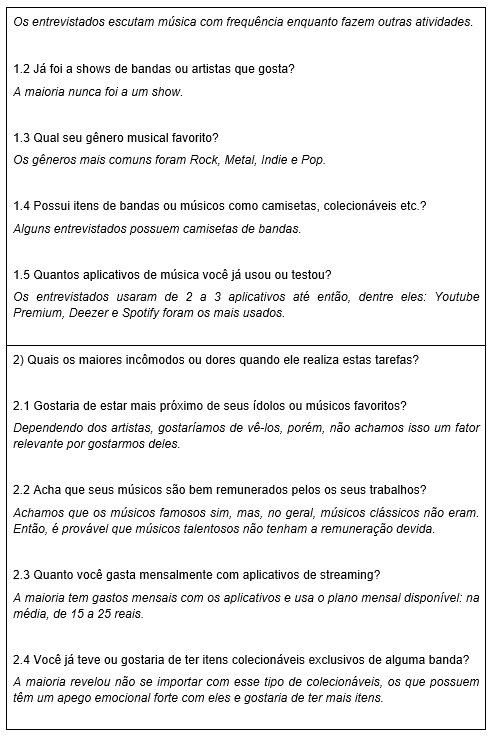
\includegraphics[width=12cm]{hs/c2.PNG}
    \caption{Resumo das Entrevistas com Consumidores. Fonte: os Autores. Parte 2 de 3.}
    \label{fig:hs6}
\end{figure}
\FloatBarrier

\FloatBarrier
\begin{figure}[h]
    \centering
    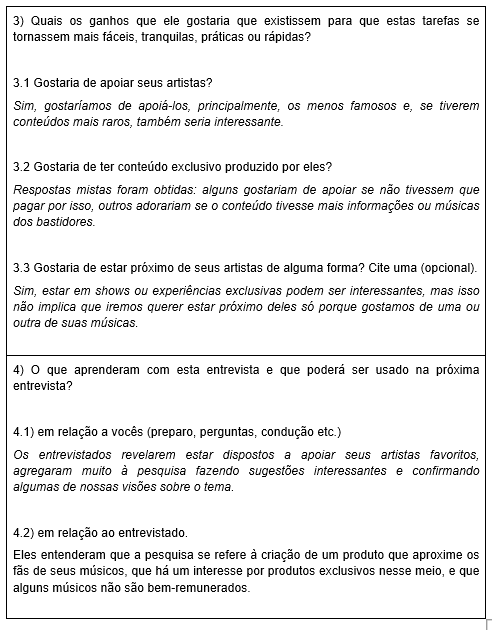
\includegraphics[width=12cm]{hs/c3.PNG}
    \caption{Resumo das Entrevistas com Consumidores. Fonte: os Autores. Parte 3 de 3.}
    \label{fig:hs7}
\end{figure}
\FloatBarrier

Com base nas informações obtidas das entrevistas, elaboramos o conteúdo das duas próximas seções, perfis mais coerentes com o mercado e os seus atores, e novos processos para o projeto ter sucesso. Os questionários e suas perguntas foram replicados para cada entrevistado, as respostas apontadas acima estão sintetizadas e representam a opinião majoritária da amostra; os nomes foram preservados, no total, foram 17 entrevistados: 8 músicos e 9 consumidores.

\subsection{Inovação de Valor (Matriz de Valor)}

Analisamos os atributos descritos nas seções anteriores e comparamos o nosso projeto com as empresas do setor para dimensionar o nosso posicionamento sobre ele, avaliando a nossa performance para propor uma estratégia de marketing eficiente.

\FloatBarrier
\begin{figure}[h]
    \centering
    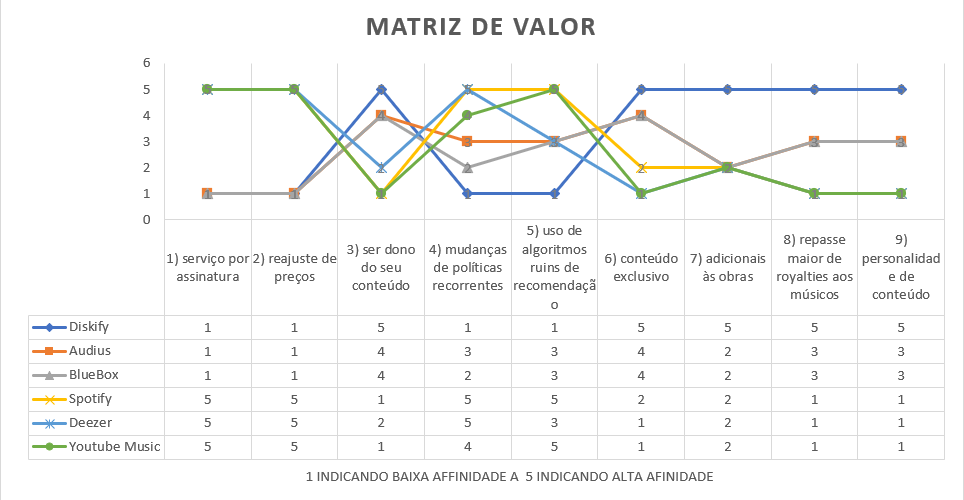
\includegraphics[width=15cm]{hs/matrz.PNG}
    \caption{Matriz de Valor.}
    \label{fig:hs1}
\end{figure}
\FloatBarrier

\subsection{Estratégia de Marketing (7P´s)} 

Para desenvolver a nossa estratégia de marketing voltada aos 7 Ps, utilizamos o conhecimento do perfis consumidor e músico; vale ressaltar que, para nós enquanto empresa, o músico também é nosso cliente e precisamos desenvolver um produto (plataforma) para que ele possa negociar os seus produtos (NFTs). Portanto, descrevemos o perfil do consumidor primeiramente e o do músico em sequência.

Para o nosso consumidor, o produto (P1) se dá por NFTs de álbuns de música que podem conter apenas a nova produção artística de uma banda, artista ou,  também, entrevistas e backstages; há também a disponibilidade de passes Vip em NFTs para shows e eventos, emitidos pelos músicos, banda para a sua performance; e a equipe Diskify estuda a possibilidade de inserção de conteúdo de podcasts em NFT para seus usuários (uma forma de remunerar os produtores de podcasts menores, que não possuem lucro com a atividade). O preço (P2) pelo nosso produto não é consensual e objetivo, na realidade, todos os preços são subjetivos - a questão, porém, é que cada álbum terá um preço seu atrelado conforme o valor que os usuários acordarem ser -, por isso, é um ambiente de muita prosperidade, onde os usuários certamente encontrarão obras não tão exclusivas por preços acessíveis. O ponto de venda (P3) se dará através de nosso domínio web diskify.nft ou através de nossos aplicativos mobile, acessível de todo lugar com internet. A promoção (P4) de nosso conteúdo será feita de forma mista e bastante livre, o músico que realiza o processo de mint do seu álbum em NFT poderá divulgar suas obras nas suas redes sociais, já trazendo um público leal à plataforma, mas haverá a possiboilidade de o músico pagar um bônus à plataforma para que seu projeto fique em destaque em uma das páginas da aplicação, ou através de marketing próprio da Diskify, escolhendo alguns álbuns para realizar a sua campanha enquanto empresa; isso tudo virá ao cliente de forma promocional, mas uma vez que um cliente poderá vender seu NFT a outro cliente, essa promoção pode ocorrer fora de nossas redes ou plataforma, com o marketing inter-pessoal. A evidência física (P5) dos NFTs negociados se dará de duas formas: 1) o músico é conhecido e promoveu sua NFT com os meios de promoção (um fã talvez avalie com muito valor, para um não-fã, talvez seja só mais um artista); e 2) o próprio preço subjetivo da obra evidencia o valor atrelado a ela, de forma a dizer que - se uma obra tende a ser vendida por preços baixos - o caráter exclusivo e qualitativo dela não é tão alto como esperado por clientes prévios, evidenciando o valor dela então. Os processos (P6) que o cliente entende de nossa empresa são bastante abstraídos de sua complexidade inerente de um projeto web 3.0, marketplace on-blockchain, de forma que o cliente o entende como adentrar uma loja de discos antiga e escolher um álbum de seu gosto (que fora posto ali alguns minutos antes pelo próprio artista) e que, caso tenha enjoado do álbum ou não tenha gostado, ele pode vir à loja e negociar com clientes que talvez tenham interesse obter aquele disco. As pessoas (P7) são endereços na rede que tiveram passado na plataforma ou a conhecem e ainda não adentraram (neste caso, seria um marketing de conquista e menos de conhecimento ou evidência física sobre as obras), os clientes com passado transmitiriam sua persona e seus gostos musicais com base na sua posse atual ou no histórico de posse (pois, poderá revendê-los), esses clientes estão disponíveis para contato - se assim o desejarem, a privacidade deles nos é importante - com base nos seus links armazenados pelo nosso smart contract na própria blockchain, sim, fizemos um mapeamento descentralizado de informações adjacentes ao álbum para fins como este; caso o cliente não encontre alguém próximo, no marketplace ou entre em contato com o músico em suas redes, ele poderá no servidor da nossa comunidade para conversar com os clientes que por lá se encontrarem e tirar suas dúvidas (planejamos o marketplace também voltado ao aspecto comunidade).

Para o nosso músico, artista ou banda, em muito se assemelha o seu comportamento de interação com a plataforma com o do cliente-fã - pois a desenhamos para ser um meio de fácil utilização para o artista também e baixa complexidade ou políticas restritivas -, o produto (P1) do músico é o marketplace e suas funcionalidades, quanto alcance ele consegue por nossas ferramentas para atingir seus fins de auto-divulgação e financiamento, pois é ele que define o preço inicial (bid) por cada unidade exclusiva (one of a kind) de seus álbuns NFTs, então ele pode estipular uma margem de lucro inicial. O preço (P2), como mencionado antes, será definido pelo próprio músico a receber pela sua produção, no entanto, há um custo de taxas a recair sobre ele na fase de mint da sua produção em NFT: essas taxas são relacionados ao processo de adicionar/modificar o status da blockchain, nosso contrato otimizou esse processo para evitar custos exacerbados; portanto o músico para por emitir um token para o seu álbum e algumas gas fees para realizar a operação na blockchain (isso tudo, por comparação com galerias NFTs, deve-o custar em torno de 10 dólares por todas as emissões). O ponto de venda (P3), nesse caso, por falta de coerência semântica, não existe para o músico, pois ele é quem anuncia sua obra no nosso marketplace; portanto, o ponto dele é o mesmo do cliente-consumidor: diskify.nft ou a aplicação mobile. A promoção (P4) do músico foi descrita no mesmo tópico do cliente-consumidor no parágrafo anterior e é a mesma para ambos, invertendo os atores da dinâmica da promoção apenas. A evidência física (P5) é bem parecida com a descrita no consumidor também, no entanto, vale ressaltar que, para o músico, a evidência recai sobre a sua reputação: quanto menor for a qualidade de seu trabalho, menor será seu apreço pelos consumidores. Os processos (P6), também, são parecidos com os descritos no parágrafo anterior, porque será essa visibilidade transmitida aos nossos artistas-parceiros, logicamente, eles estarão mais a par do funcionamento de royalties e algumas outras funcionalidades da plataforma que os clientes talvez não tomem razão sobre; todo o processo de emissão, lógica de vendas e preços é o mesmo para ambas personas por conseguinte. As pessoas (P7), no caso do músico, são um escopo maior, pois temos a intenção enquanto empresa de favorecer a comunicação entre os artistas para fomentar o surgimento de colaborações entre produções para a plataforma, nessa tentativa de aumentar o estoque de produtos no marketplace também estimulamos o contato e suporte entre os produtores, criando essa rede de ajuda e comunicação pela internet; mas, também, possibilitamos o alcance de novos seguidores as suas redes e perfis através de promoção de suas obras no nosso marketplace.

\subsection{Previsão de Demanda} 

Para estipular nossa demanda, avaliamos apenas o número de consumidores possíveis na rede adeptos à ideia do projeto no começo. Como apontado nas notícias, o número de endereços ativos na rede Ethereum é de 1,65 milhão\cite{finb}. Pegaremos a parcela dos entrevistados consumidores adepta à nossa ideia, 78\% (7/9), e multiplicaremos pelo número de endereços; temos 1,28 milhão de prováveis endereços consumidores. Para entender o capital possível de atingir, faremos uma regra de proporção, analisaremos o valor do mercado de nova iorque, NYSE, e o resultado da indústria músical e compararemos com o valor da rede Ethereum. Sobre o mercado da música, ele cresceu 9.7\% de 2017 para 2018\cite{ubcm}, valendo US\$ 19.1 bilhões, fizemos o cálculo a valor presente para 2021, mantendo o mesmo crescimento (para fins de facilitação do cálculo) e obtivemos US\$ 25.21 bilhões para 2021 aproximadamente. A bolsa, durante 2020 e 2021, fez o movimento de retomada em V devido à pandemia, consideraremos o valor de 5 de maio de 2020 dessa matéria\cite{nyse}, US\$ 21 trilhões de valor. Para a rede Ethereum pegaremos o valor atual, que é equivalente ao patamar de 2021 (o mercado está em recesso), US\$ 362 bilhões\cite{coim}. Realizando a proporção, obtemos que o mercado vale US\$ 329 milhões. Como somos o único aplicativo na rede Ethereum a fazer isso e levamos em conta apenas o valor dela no mercado cripto, temos possibilidade de obter 100\% do mercado. 

Vale ressaltar que fizemos o cálculo com base em endereços consumidores (fãs) e não endereços produtores (músicos), isso porque a nossa pesquisa revelou que todos os músicos entrevistados não teriam problemas em pertencer a este meio, na verdade, para eles a parte de negociação de suas produções é tão restritiva que causa um desânimo neles e os impede de pensar para este lado do mercado, os motiva a fazer parte também - pois não têm amarras com o mundo 2.0. Podemos, também, considerar o caso citado na introdução para o mundo das artes, o quadro foi leiloado por 69 milhões de dólares, isso nos motiva a crer que, mesmo com um número baixo de produtores, é possível rentabilizar bastante; note que a uma grande dissonância entre o potencial do nosso mercado e o preço dessa única obra, isso se dá porque o mercado musical ainda é praticamente inexistente na web 3.0 e porque a maior parte do capital dessa compra estava em endereços não tão ativos da rede, sem contar o capital que pode ser obtido de outras redes blockchains e, até mesmo, do mundo convencional através de crédito pelo nosso framework de pagamentos auxiliar, moralis, ao smart contract desenvolvido por nós: possibilitando a junção de vários pontos de capital para efetivar uma única compra.

\section{Viabilidade Técnica}

Sobre a viabilidade do projeto {\it Diskify}, conciliamos os pontos descritos nas seções acima de forma técnica; vale ressaltar que nossa empresa se difere do usual no que tange operabilidade, pois é uma DAO (do inglês, organização autônoma descentralizada) - isso significa que ela deve operar com o mínimo de pessoas no molde empresa tradicional e o máximo de usuários na rede atuando sobre os nossos contratos inteligentes para dar vida a empresa, assemelhando-se bastante com comunidades. E essa é uma de nossas intenções: tornar o projeto em uma comunidade ativa de somente fãs e músicos, descreverei melhor o ponto com relação aos profissionais, suas tarefas e longevidade na organização a seguir.

\subsection{Produção / Operação}
 
Os detalhes da produção foram descritos na seção 4, os componentes da aplicação serão declarados de forma passo a passo conforme a aplicação foi arquitetada para ser.
 
O projeto se baseia na arquitetura orientada a serviços (SOA). Para que o MVP seja concluído, a plataforma Diskify foi desenvolvida em 7 etapas, cada uma consistindo na construção de um grupo de componentes da arquitetura. 

Na primeira etapa, foi definido as bases do banco de dados da aplicação. Utilizaremos recursos da linguagem Solidity para mapear os dados entre diversos contratos inteligentes na rede. Neles foram salvas as músicas de um disco e identificadores de contratos inteligentes para o download dos conteúdos e reprodução no player.

Na segunda etapa, foram construídos os componentes de lógica de negócio: um gerenciador de criação de Smart Contracts (estrutura que possibilita a criação de NFTs), um componente responsável por postar os arquivos de músicas na base de dados, e um componente responsável por delegar as criptomoedas à rede da Ethereum (Moeda usada pela aplicação para efetuar as transações); este componente é utilizado para prover liquidez à rede se o músico assim desejar e, com isso, criar um canal para aumento das recompensas que ele recebe e, também, um meio de aumentar a receita do projeto. No desenvolvimento desta etapa, a linguagem Solidity (linguagem usada para criação de contratos na rede) foi usada para a criação dos contratos em conjunto com o Node.js.

Na terceira etapa, os componentes de uso por parte da persona consumidor foram desenvolvidos, são eles: o componente de busca de discos, um componente que realiza as ações de compra, e outro para o download do conteúdo em seu player. Estes componentes foram desenvolvidos em Node.js, à exceção do componente para download que será desenvolvido depois do MVP para dispositivos mobile, mas que consta aqui para motivos de explicação do funcionamento da lógica da aplicação.

Na quarta etapa, foi integrado à plataforma os componentes de auditoria e permissão de novos músicos e componente de gerenciamento de contas; ambos foram manipulados por membros da Diskify e foram desenvolvidos em Node.js com o auxílio de outras linguagens ou frameworks.  

Na quinta etapa, foram criadas as páginas da aplicação web em Node.js. Cada página foi tratada como um componente da aplicação, sendo elas: a página inicial da aplicação, a página de informações do usuário, a página de pesquisa por álbuns, a página de publicação de conteúdo de acesso restrito a músicos e a página de compra e pedido de compra de um disco. 

Na sexta etapa, foi desenvolvido a espinha da aplicação que coordena os componentes e interconecta as páginas, provendo funcionalidade à aplicação. Este componente é conhecido em arquiteturas SOA como Enterprise Service Bus (ESB), que é responsável por encaminhar os pedidos e gerenciar requisições de serviços. Este componente foi desenvolvido em Node.js. Os componentes da segunda a sexta etapa estarão em um mesmo servidor que ofereça suporte ao framework escolhido.

Na sétima etapa, foram realizados testes de integração e performance da aplicação em nuvem.

Os resultados foram validados ao fim de cada etapa com testes de compatibilidade e integração ao algoritmo desenvolvido. Ao término das etapas citadas conforme o cronograma proposto, caso haja espaço de tempo para integrar outras soluções em NFTs para dores de músicos e consumidores como apontado na seção 2, adicionaremos ao MVP a possibilidade de oferta e compra de passes VIP para o backstage de shows. A lógica deste produto foi explicitada, também, na mesma seção.

Para fins de consolidação da estrutura da aplicação, a próxima figura demonstra a visão proposta e referenciada nesta subseção por etapas.

\FloatBarrier
\begin{figure}[h]
    \centering
    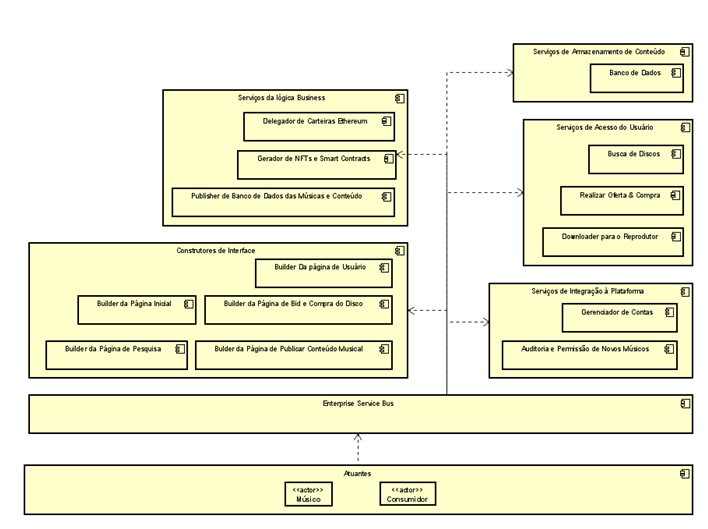
\includegraphics[width=15cm]{hs/ad1.PNG}
    \caption{Arquitetura Orientada a Serviços do Projeto Diskify. Fonte: os Autores.}
    \label{fig:la2}
\end{figure}
\FloatBarrier

\subsubsection{Detalhamento do Produto / Serviço}

Discutimos na introdução e no marketing, os motivos que tornam o mercado de Criptoativos e soluções relacionadas à área atraentes ao público, bem como a diferença entre valor e preço, objetivo e subjetivo: tópicos relacionados à economia que, juntos das soluções digitais, servem como uma nova forma de se armazenar valor e facilitar trocas, dando ao indivíduo maior poder sobre seu capital, subsequentemente, tornando mais livre economicamente. Mostramos que o cenário comprador está favorável à aplicabilidade da tecnologia NFT, e que o projeto visa a integrar a primeira arte ao futuro do comércio de bens de propriedade intelectual: obras, músicas etc. 

Temos em vista diminuir a distância entre o artista, músico de seu fã, proporcionando colecionáveis a este e uma fonte alternativa àquele.

Com a plataforma proposta, os artistas podem vender álbuns – havendo um limite de cópias definido pelo artista, o que aumenta a raridade do produto –, eliminando a porcentagem da receita líquida que vai para as gravadoras e gerando uma fonte de renda alternativa para que não dependam de seus shows apenas. Como há uma raridade em cada álbum, fãs podem acordar um preço pelo produto de forma subjetiva – pois a plataforma Diskify em muito se assemelha à uma Exchange de valores ou um Marketplace digital – e, se a posteriori decidirem revendê-los, haverá um mecanismo conhecido como royalties utilizado em NFTs de arte digitais: é uma forma de recompensar o artista pelo seu trabalho, a cada troca feita uma porcentagem do preço acordado é repassada ao músico. 

\subsubsection{Processo de Obtenção do Produto / Prestação do Serviço}

O projeto Diskify é uma plataforma de livre acesso e negociação de bens digitais que possibilita trocas de álbuns musicais por criptomoedas, integrando o direito de propriedade sobre o álbum em NFTs e as armazenando em carteiras digitais cripto, se o usuário assim desejar. Com uma NFT, o fã pode baixar para seu dispositivo as músicas e reproduzi-las, mas, caso queira revender seu token, as terá removidas de seu dispositivo. Isso não impede que algum usuário regrave as músicas e as poste em alguma outra plataforma, mas isso configura pirataria e continuará sendo um item de menor valor subjetivo do que o original. Abaixo, segue-se o modelo que mantém a lógica do produto proposto.

\FloatBarrier
\begin{figure}[h]
    \centering
    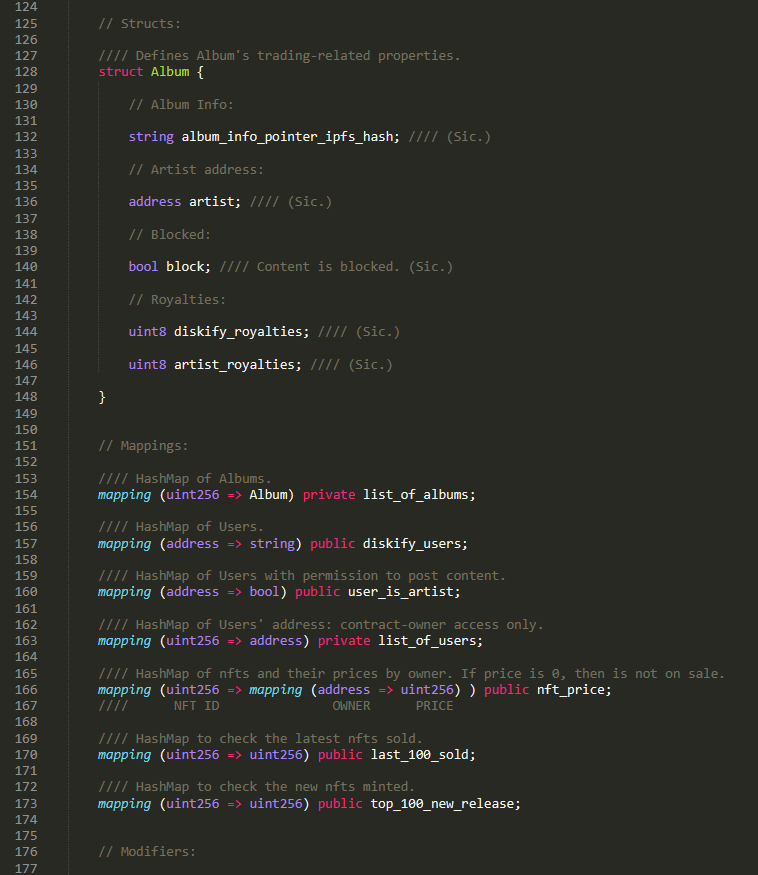
\includegraphics[width=15cm]{ks/album.PNG}
    \caption{Molde do produto. Fonte: os Autores.}
    \label{fig:la1}
\end{figure}
\FloatBarrier

Como pode observar, os conteúdos do objeto struct na linguagem Solidity foram ainda mais abstraídos por questões de reduções das gas fees na ação mint. Isso significa que os dados de álbum: músicas, nomes das músicas e dos compositores, capa etc. estão armazenados em uma segunda blockchain, dedicada ao armazenamento de dados - na rede Ethereum, persistirá apenas os dados relacionados às transações feitas com a posse do número serial de um álbum em questão e seu ponteiro-hash para a segunda blockchain, onde está armazenado em conteúdo. E, sobre os mappings (eles dão uma ideia sobre o fluxogramas a seguir), são HashMaps dos valores a si endereçados para encontrá-los através da rede, pois ela é distribuída e descontinuada em muitos blocos, necessitando um ponteiro que indique o caráter único do álbum. 

\paragraph{Fluxograma dos Processos de Obtenção do Produto} $\\$

Sobre a obtenção:

\FloatBarrier
\begin{figure}[h]
    \centering
    
\includegraphics[width=12cm]{ks/d1.PNG}
    \caption{Diagrama de obtenção do produto.}
    \label{fig:s5d1}
\end{figure}
\FloatBarrier

\paragraph{Fluxograma dos Processos de Manutenção do Produto} $\\$

Não existe manutenção do produto oferecido, ele não sofre degradações externas: é intangível; a única mudança é quanto a sua disponibilidade: dependo do conteúdo, pode ser necessário um bloqueio de sua transmissão, essa variável inabilita os possuidores do álbum de escutá-lo - isto está no contrato e força os compradores a evitarem a compra de conteúdo com direitos intelectuais, pois isso seria um desperdício de fundos caso o álbum sofresse algum bloqueio. Detalhe importante: sobre o conteúdo, uma NFT deve manter seu estado para preservar o valor, portanto, não há mudanças no álbum com relação ao seu conteúdo exclusivo, o músico até pode mudar suas características: fotos, descrição, planos da banda etc. - e eles apareceriam na página de apresentação do álbum e seu conteúdo não-exclusivo - mas não participariam do conteúdo inerente ao álbum. Logo, as mudanças no álbum descritas abaixo, não estão salvas nele e são com relação a esse espectro descrito, isso é mais pela necessidade de explicar o modelo de negócio neste fluxograma.

\FloatBarrier
\begin{figure}[h]
    \centering
    
\includegraphics[width=12cm]{ks/d2.PNG}
    \caption{Diagrama de manutenção do produto.}
    \label{fig:s5d2}
\end{figure}
\FloatBarrier

\paragraph{Fluxograma dos Processos de Prestação do Serviço} $\\$

Esse é modelo de prestação de serviços da empresa, observe que não interferimos no que o usuário está motivado a fazer, nosso trabalho é de suporte no máximo - fora toda a parte de competência técnica.

\FloatBarrier
\begin{figure}[h]
    \centering
    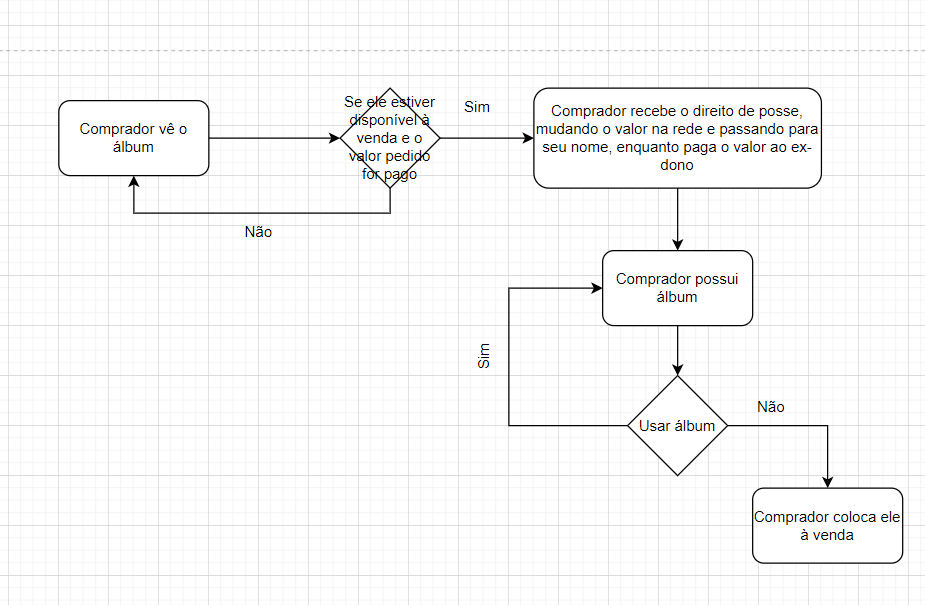
\includegraphics[width=15cm]{ks/d3.PNG}
    \caption{Diagrama de manutenção do produto.}
    \label{fig:s5d3}
\end{figure}
\FloatBarrier

\subsubsection{Tecnologia, Máquinas e Equipamentos}

A aplicação Diskify utiliza duas blockchains para executar a sua lógica de negócios. Foram usadas a rede Ethereum para a parte de negociações de NFTs entre as personas e armazenamento dos preços dos álbuns, bem como os dados das transações, por ser uma dApp (Aplicação Descentralizada), cada estado do contrato inteligente está fixado na cadeia de blocos; e a rede IPFS (Inter-Planetary File System) para armazenar o conteúdo de um álbum, como as músicas e a capa. O uso de duas blockchains se dá justamente para utilizar os pontos fortes das redes de forma eficiente e com baixo custo de transferência (taxas de transação: gas fee): na rede Ethereum, o custo para salvar os bytes de dados de uma música seriam altos, portanto, a utilizamos para realizar movimentações de tokens, checar o balanço das contas, fazer emissão de novas NFTs e organizar os dados dentro dos objetos a cada estado do contrato após a execução de alguma de suas funcionalidades. Para emitir um álbum em NFT, o endereço (pessoas são definidas na rede como um endereço) deve pedir aprovação para se tornar artista ao contrato da aplicação na rede Ethereum, que é responsável pela lógica de negócios e atua como um servidor para a aplicação; esta permissão é um mecanismo para prevenir o spam de conteúdos por pessoas não autorizadas. Logo após emitir um contrato, a aplicação front-end, feita em Node.js, se encarregará de exibir a NFT à venda nas páginas do aplicativo (caso haja alguma cópia disponível – se o preço estiver definido como 0, então não está à venda e a aplicação apenas mostrará as informações do álbum existente na rede, mas impossibilitará a negociação dele), dessa forma o usuário poderá conhecer NFTs e negociá-las. A aplicação está descrita em seu funcionamento base, no entanto, ressaltamos que: utilizamos a carteira digital Metamask para conectar endereços na aplicação e habilitar as negociações.

Os preços das NFTs negociadas são definidos pelos seus donos e uma transação só ocorre se as duas partes aceitaram o preço acordado. O número de cópias de um álbum é definido pelo músico que o emitiu na rede, sendo esse número de álbuns disponíveis à venda. A cada transação são emitidos royalties à Diskify e aos músicos, esse percentual e definido pelo músico na emissão da NFT e, a cada transação, o percentual do preço negociado é enviado às carteiras definidas dos músicos e da Diskify automaticamente pelo contrato inteligente. A aplicação utiliza diferentes paradigmas na sua arquitetura: o acesso aos dados é feito com base em arquitetura micro-serviços; o contrato inteligente opera com base no paradigma funcional e decoradores que modificam o curso de execução das funções conforme os requisitos necessários por parte de quem chama a função – ou seja, impede, com redundância, que estados indesejados existam durante a execução, mesmo que o front-end altere a chamada da função; e o front-end utiliza orientação a objetos e o paradigma funcional para gerar página reativas e não necessitar de dados externos às blockchains para o seu funcionamento. Contudo, os contratos, após entrarem na rede blockchain (deployment), não podem ser alterados – uma característica que garante confiabilidade ao aplicativo desenvolvido –, nem mesmo pelo o programador que o desenvolveu; por isso, a parte front-end é o ponto crítico na aplicação com relação a cerceamento da aplicação, porém, uma vez na rede, o contrato pode ser usado por diferentes usuários (mantendo os endereços e royalties aos usuários na rede), logo o front-end se torna um ponto de acesso centralizado à aplicação descentralizada, podendo, assim, ser refeito e sofrer alterações para utilizar o mesmo contrato – o que o torna maleável para mudanças de interface e experiência de usuário.

\paragraph{Processos de Obtenção do Produto} $\\$

A parte de servidor da aplicação e sua lógica, e database estão disponíveis para uso nas redes blockchains e contam com as melhores máquinas para a operação. Quanto ao front-end, a parte de desenvolvimento será feita pelos nossos desenvolvedores para aprimorar o uso da comunidade e sua disponibilidade será feita em servidores terceirizados para acesso da internet à aplicação, pode - no entanto - ser feita dos computadores da empresa no futuro para melhora da eficiência da empresa, uma vez que nosso serviço apenas fornecerá páginas web iguais a usuários que, de seus computadores, se conectaram à rede, funcionando mais como um repositório dessas páginas e sendo de fácil manutenibilidade.

\paragraph{Processos de Manutenção do Produto} $\\$

Nosso produto não precisa de manutenção em servidor e em database por motivos citados quanto ao modelo de negócio; no entanto, as redes sofrem versionamento para melhora de processos na blockchain, assim como o framework moralis - todos automaticamente aprimorando o nosso negócio sem mudá-lo ou precisar. O front-end da aplicação pode sofrer mudanças, nossos desenvolvedores o criariam e, depois, uma parte menor deles seria necessária para mudar alguns detalhes, se necessário fosse. No entanto, observe que um segundo plano da empresa é não depender desse pesar: necessitar de programadores para cuidar de um front-end; para nosso caso, eles serão efêmeros - isso porque a DAO criada será aprimorada através da seção de sugestões ou dúvidas no nosso site, que apontará desejos da comunidade para o projeto, necessitando que o dono do contrato realize a mudança por eles; e note que dúvidas de usuários poderão ser respondidas por outros usuários, assim como entrar em contato se precisar e assim quiser outro usuário ser comunicado.

\paragraph{Processos de Prestação do Serviço} $\\$

Para prestar esse serviço, a empresa será o ponto de acesso único centralizado (no início) para a aplicação. A dinâmica de pagamentos pode parecer confusa, mas ainda que outra empresa use o nosso contrato e atraia clientes para seu front-end, seus custos terão que incluir o pagamento para nossa empresa, pois foi definido em nosso contrato o envio à nossa carteira, e o uso do contrato com a afinidade e preferência dos músicos garantirá seu uso para unir a comunidade em um ponto de operação único e padronizado de músicas na rede. Isso significa que incentivamos os usuários a até criarem seus front-ends mobile, por exemplo, de forma a personalizar a seu gosto - no entanto, eles só serão recomendados pela {\it Diskify} se cumprirem com nossos requisitos de uso, privacidade e anonimidade. 

Esse serviço será prestado por nós no início e, se houver a necessidade de expandir o {\it load balancer} para fornecer as páginas aos usuários e garantir o acesso aos clientes, a empresa pode pensar em usar servidores terceirizados. 

\subsubsection{Equipe Técnica}

Com relação a equipe técnica, será necessário: programadores database/servidor de blockchains (já supridos por mim); programadores front-end para aprimoramento futuro - se necessário expandir rapidamente (já supridos por mim); uma equipe de marketing inicial para a plataforma e para alguns álbuns no início - mas, provavelmente, isso será cuidado pelos próprios artistas com auto-divulgação e assistência de seus produtores (se desejarem); uma equipe para instruir o uso da plataforma e eventuais complicações e desentendimentos, preenchendo a seção de ajuda e suporte, e um número menor ainda, depois de um tempo, para resolver problemas com músicos e clientes problemáticos.

\paragraph{Processos de Obtenção do Produto} $\\$

O processo de obtenção será feito através de nosso site, esse é o melhor jeito do conquistar interessados em blockchain (programadores, entusiastas e pessoas querendo ajudar a comunidade com habilidades não-tecnológicas).

\paragraph{Processos de Manutenção do Produto} $\\$

A manutenção da equipe será feita por mim, mas caso haja a necessidade de mais coordenação das partes, um gerente poderá ser inserido para a tarefa. Não será necessário para o início do projeto administradores para cada grupo de profissionais acima citados, isso porque eu sei o que deve ocorrer em cada parte da aplicação, tecnica e moralmente.

\paragraph{Processos de Prestação do Serviço} $\\$

O serviço a esses profissionais será prestado através da rede e grupos pessoais reservados à comunicação intra-empresarial; como visamos eficiência, teremos a dinâmica de trabalho fully-remote, logo, nossos profissionais virão de diferentes lugares e a comunicação será feita em inglês (traduções de dúvidas e funcionamento da plataforma serão feitas por algoritmos, nosso conteúdo original será bem descritivo e meticuloso para evitar ambiguidades de tradução).

\subsubsection{Alinhamento da Capacidade Instalada com a Demanda} 

Como já citado, a demanda não impacta o nosso software diretamente; há a possibilidade de mudar o servidor fornecedor de páginas requisitadas para os usuários utilizarem nossos contratos inteligentes caso o número de requisições simultâneas seja alto demais e surja a necessidade de um melhor load balancer (de servidores terceirizados). No entanto, essa preocupação só será real com um número muito alto de usuários - e não será o caso início -, dificultando saber se haverá necessidade. Todo o processamento e armazenamento ocorrem nas redes blockchains e não necessitam nosso poder computacional.

\subsubsection{Localização}

Toda a parte de localização dos nossos serviços e produtos se dá por software, virtualmente, nos aplicativos mobile e em nosso site: diskify.nft, sem haver a necessidade de existirmos como negócio fisicamente.

\subsubsection{Arranjo Físico das Instalações} 

Como dito, pretendemos operar fully-remote, então, não precisaremos de escritórios ou salas comerciais; nossa estrutura está na rede e não gera muitos custos diretos altos, e eles são pagos de forma inteligente com transações entre partes, o custo do nosso front-end é o mesmo de manter um servidor repositório fornecedor de páginas web, que eu imagino ser e manter-se abaixo de 0.01\% do nosso lucro. Nossos profissionais trabalharam de casa com seus equipamentos, a empresa não terá que bancar esses custos. Toda via, criamos um mecanismo que nos permite alterar os custos por transações e ajuda a manter o percentual acima almejado para rentabilidade preferida, ou podemos encontrar alternativas custo-oportunidade melhores para o projeto.

\subsubsection{Custos}

Quanto ao custos dos profissionais, isso será relatado na seção 5.2. Sobre nossos custos com a produção: o músico cobre o custo de se tornar músico dentro do contrato inteligente e passa o valor de entrada a nós, pagando pelas gas fees da operação executada também; o músico se encarrega de produzir o conteúdo artístico, pós-término, então decide ele publicar em nossa comunidade, logo ele realiza o upload e preenchimento de dados, nesta fase, ele modifica o contrato - criando um novo token e um novo balanço de unidades (essa operação tem custos dentro de uma blockchain, pagos aos mineradores em forma de gas fees maiores, no entanto, tomei cuidado de reduzir o custo ao máximo) e armazenando os dados do álbum na blockchain dedicada, para realizar este serviço, teremos de contratar os planos do serviço infura.io (o plano com mais atributos custa US\$  1000 ao mês, que é bem conveniente - entraremos em contato se precisarmos de um serviço mais robusto) -; quanto aos custos de transações entre clientes pós-lançamento do álbum, os custos de modificação da blockchain recaem sobre o preço que o cliente comprador paga - nos deixando sem custos quanto a isso. Para manter o front-end repositório, checamos os preços e - para tal tarefa - gastaremos em torno de BRL 1000 ao mês. Quanto a manter o produto, os músicos e compradores podem mudar dados pessoais dentro da blockchain, esse custo é muito baixo, mas é encoberto por eles. Abaixo estão ressaltados todos os custos com relação ao produto e o que a empresa terá que despender. Descrevi todo o processo de obtenção aqui e nas seções acima, colocarei apenas o sumário de custos dos processos nas subseções abaixo. A empresa despenderá, mensalmente, com custos de produção, algo até US\$ 1500 na expectativa de um cenário de pior caso, e, segundo os cálculos, US\$ 1200 para manter todo o funcionamento da produção.

\paragraph{Processos de Obtenção do Produto} $\\$

\begin{longtable}[c]{|l|l|} \hline
\textbf{Tarefas}                                 & \textbf{Custos da {\it Diskify}} \\ \hline
\endhead
%
Criação do token do álbum no contrato            & 0               \\ \hline
Publicação do conteúdo na 2a blockchain dedicada & 0               \\ \hline
\textbf{Total (US\$):}                           & \textbf{0}      \\ \hline
\caption{Custos de Obtenção do Produto}
\label{tab:tc1}\\
\end{longtable}

\newpage

\paragraph{Processos de Manutenção do Produto} $\\$

\begin{longtable}[c]{|l|l|} \hline
\textbf{Tarefas}             & \textbf{Custos da {\it Diskify}} \\ \hline
\endhead
%
Mudar informações da persona & 0               \\ \hline
\textbf{Total (US\$):}       & \textbf{0}      \\ \hline
\caption{Custos de Manutenção do Produto}
\label{tab:tc2}\\
\end{longtable}

\paragraph{Processos de Prestação do Serviço} $\\$

\begin{longtable}[c]{|l|l|} \hline
\textbf{Tarefas}                           & \textbf{Custos da {\it Diskify}} \\ \hline
\endhead
%
Manter blockchain de armazenamento         & 1000                       \\ \hline
Manter servidor repositório de páginas web & 200                        \\ \hline
\textbf{Total (US\$):}                     & \textbf{1200}              \\ \hline
\caption{Custos de Prestação do Produto}
\label{tab:tc3}\\
\end{longtable}

\subsubsection{Sistemas de Gestão da Qualidade}

Nossa qualidade se dá pelo serviço prestado com o melhor custo-benefício do mercado a todas as partes envolvidas, o software backend é optimizado para resolver todas as necessidades da empresa agora e pensado para resolver 90\% de tudo que precisará no futuro. Como dissemos, nosso projeto é uma DAO e presa pelo consenso da comunidade sobre o funcionamento - quanto às dúvidas de operação, lógica de negócio e problemas eventuais, nossa própria comunidade poderá interagir entre si para esclarecer o melhor uso de nossa plataforma e como contornar possíveis frustrações, assim como sugestionar melhorias e ideias para o aplicativo, como, também, poder programar soluções de frontend e pedir aprovação da nossa DAO para interagir com o nosso aplicativo. Usaremos a ideia de mecanismo de aprovação e qualidade usado no site {\it Silk Road}: aprovação por rating de qualidade de serviço prestado ao usuário pelo usuário em escala de qualidade de 1 a 5 para álbuns e soluções diversas na plataforma.

\subsection{Gestão de Pessoas}

Somos bem diretos quanto a empresa e trabalho: temos problemas, se você é capaz de resolvê-los a tempo hábil e ser performático, está apto a ser parte do projeto {\it Diskify}. Faremos gestão de pessoas por competência, nosso modelo fará com que os profissionais se comprometam com a comunidade e com o objetivo da DAO.

\subsubsection{Competências}

Quanto a competências genéricas, nossa filosofia nos diz que quem possui os requisitos técnicos abaixo descritos é competente o suficiente para entender as atitudes da empresa e por que nos existimos. Mas vale ressaltar que afiliaremos ao projeto as pessoas que tenham visão política-social, habilidades de programação mínimas, boa retórica, conhecimento econômico e nível muito avançado em inglês; não nos importamos com burocracia de recrutação ou com a ideia vaga de ser polido nos termos para não dar entendimento exato aos profissionais do porquê não são aptos a atuar. Para aqueles que possuem as nossas habilidades descritas, nenhuma descrição a mais é necessária sobre conduta.

\FloatBarrier
\begin{figure}[h]
    \centering
    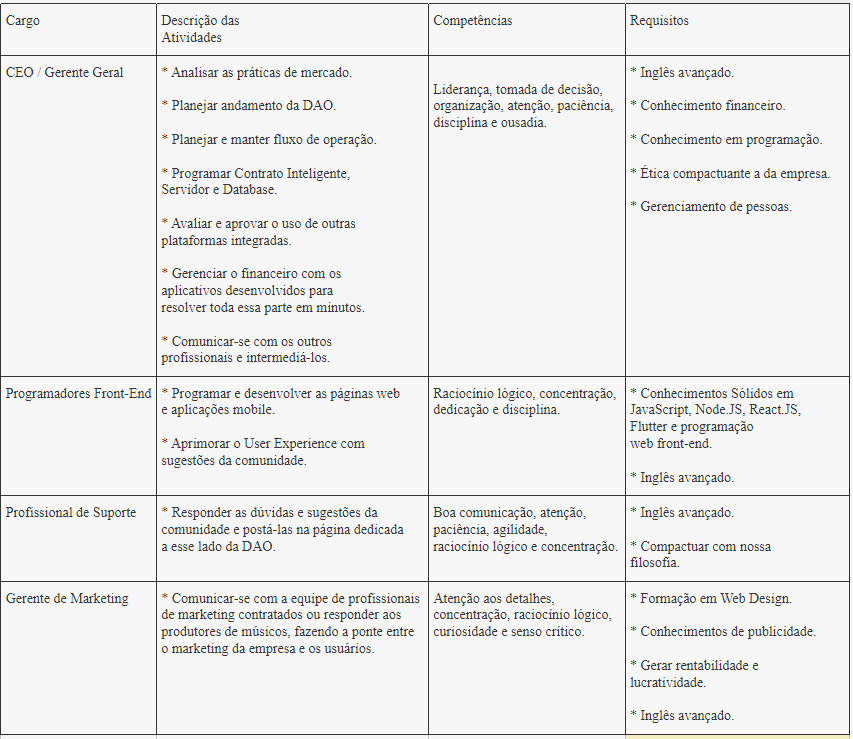
\includegraphics[width=15cm]{ks/compd.PNG}
    \caption{Competências específicas {\it Diskify}.}
    \label{fig:compd}
\end{figure}
\FloatBarrier

\subsubsection{Estrutura Organizacional}

Cada responsável no organograma abaixo cumpre as atividades descritas na seção anterior passo a passo; precisamos de alguns poucos bons profissionais, encontrá-los se dará por intermédio do crescimento orgânico da comunidade, não existe muita diferença de valor entre diferentes tipos de atuação, fora o fato de que todos respondem ao CEO gerente-geral, e ele comunica-se com todos para o andamento da empresa: não faremos distinção em níveis portanto.

\paragraph{Organograma} $\\$

\FloatBarrier
\begin{figure}[h]
    \centering
    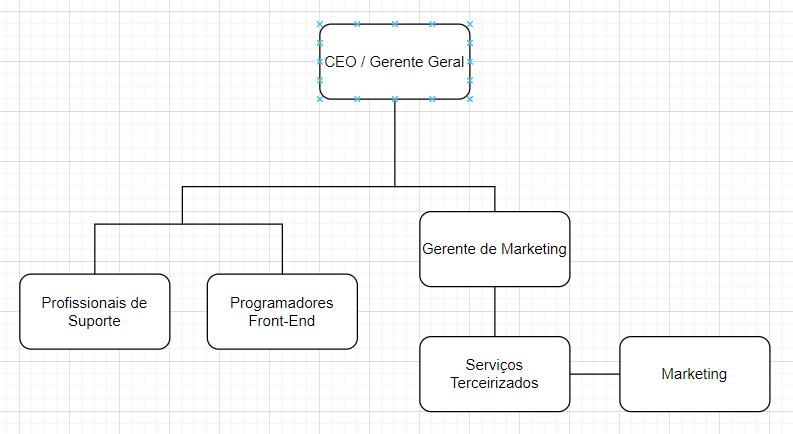
\includegraphics[width=13cm]{ks/hierarquia.PNG}
    \caption{Organograma da dinâmica de trabalho da {\it Diskify}.}
    \label{fig:hierarquia}
\end{figure}
\FloatBarrier 

\paragraph{Pessoal} $\\$

O CEO gerente-geral é encarregado de conciliar todos os profissionais e dá-los sub-tarefas para cumprir com suas obrigações e ajudar no planejamento idealizado pelo CEO, ele analisará as práticas de mercado, planejará o andamento da DAO, mantendo o fluxo da operação, manterá o devido cuidado quanto a lógica de servidor da aplicação enquanto programa os contratos inteligentes da aplicação - que são o servidor e a database dela ao mesmo tempo; ele poderá conceder direito de uso a plataformas que desejem se integrar a aplicação contanto que elas cumpram com os requisitos definidos pela a organização; ele cuida do financeiro pois tem toda a dinâmica dele definida por plataformas inteligentes que conseguem conciliar tudo em um só lugar; vale ressaltar que muitas dessas atividades são realizadas uma vez na existência da aplicação, pois os contratos devem remanescer inalterados de forma a garantir boas práticas de conduta pela comunidade, logo a carga do CEO diminui com o tempo ao passo que fica automatizada, e ele passa a apenas gestar a DAO - é ele quem se comunica e define os planos de aprimoramento para os profissionais contratados, avalia seus resultados e os integra.

O profissional de front-end realiza as atividades de melhora visual e experiencial da plataforma com base nas sugestões de usuários e demandas do CEO para interação com o contrato de forma eficiente; também, conciliando com baixas solicitações ao servidor repositório pelos usuários, ele fará as versões das aplicações mobile também. O profissional de suporte responderá às dúvidas dos usuários na aplicação e melhorará a qualidade da comunidade, poderá produzir conteúdo informativo e auxiliar usuários com eventuais dúvidas na plataforma.

O profissional de marketing escutará as necessidades do CEO e as aplicará de forma mercadológica na aplicação anunciando ela a novos parceiros e promovendo-a a novos consumidores; ele entrará em contato com possíveis produtores de músicos e resolverá o problema ele mesmo ou os encaminhará ao pessoal de suporte.

\paragraph{Terceirização} $\\$

Quanto a terceirização, o gerente de marketing poderá pedir verba ao CEO para contratar times de marketing para promover campanhas em nome da organização até que ela se popularize ou em tempos de oportunidade para expansão, o uso desses profissionais pode ser esporádico; basicamente, atuarão na parte de design propagandístico. Os custos da terceirização deverão variar e não devem ser levados como um grande problema, pois manteremos 5\% da lucratividade mensal em propaganda no máximo.

\subsubsection{Recrutamento e Seleção}

O processo de recrutamento será feito de forma flexível através da plataforma por usuários competentes que queiram contribuir com o projeto; será passado algumas tarefas para que resolvam e, se os resultados, seus portfólios e perfis, forem coerentes serão recompensados por tarefa e ganhando o direito de preferencialidade para resolução de problemas na plataforma. Algumas vagas podem ser divulgadas em sites de trabalho remoto. Para quem está na comunidade, tem a capacidade de atuar no projeto e quer, nenhum excesso em recrutamento é necessário, é bem provável que será competente para realizar tarefas be baixo impacto funcional no projeto (pois essas já foram feitas pelo CEO na maturação do projeto), participando no lado mais favorável aos gostos visuais e experienciais dos usuários da comunidade.

\subsubsection{Treinamento e Desenvolvimento}

Para os programadores e profissionais de marketing, conhecimento de suas competências não serão necessários - e eles escutaram as ideias da comunidade sobre planos futuros, obtendo um rumo dessas sugestões. Para os profissionais de suporte, conhecimento apenas sobre a filosofia da empresa e como melhor proceder em certos cenários (isso segundo o CEO) - pois sua área de atuação será resolver problemas da comunidade postadas na área de sugestões.

\subsubsection{Remuneração}

Sobre a remuneração, haverá um espaço de sugestões na plataforma onde clientes-fãs ou consumidores poderão pedir por recursos na plataforma e postar uma recompensa para quem entregar o trabalho pedido; esses pedidos serão elencados por nós para serem aplicados na plataforma e, então, qualquer programador poderá prototipar os recursos conforme nossos requisitos e obter a recompensa da comunidade. Quanto aos nossos profissionais, eles serão obtidos dessa forma, caso haja interesse em tê-los como desenvolvedores ativos-fixos da DAO, eles receberam uma porcentagem do lucro mensal como remuneração mensalmente. 

Sobre a ideia de que seu trabalho deve ser sua realização e tudo nele deve ter uma sala colorida para questionar por quês relativos... achamos desnecessário ressaltar que tudo isso é ineficiente e vai contra a nossa filosofia e comunidade - portanto, diferente do sistema convencional de empresa e de contratação, nós não teremos cuidados com extras na remuneração de nossos profissionais (a ideia é remunerá-los pelo o que fazem na DAO e apenas isso). Sobre valores de taxas incidentes às remunerações, ressaltamos que somos, expressamente, contra essas políticas e faremos o máximo para não contribuir - um dos motivos de pagarmos com os próprios cripto-ativos -, logo, não consideramos taxas sobre os pagamentos; no entanto, os profissionais podem ter descontos desses caso realizem algumas movimentações de capital.

Na tabela abaixo, consideramos os preços atrativos para manter com cada categoria de atuação na plataforma. O percentual para grupo resume o montante despendido com eles do lucro mensal obtido; para grupos com 4 profissionais, o total percentual do grupo será divido entre eles igualmente. Alguns bônus podem ocorrer para eventuais tarefas definidas pelo CEO e que sejam cumpridas em tempo hábil. Consideramos os custos de manutenibilidade e de propaganda para fecharmos o cálculo da tabela (que fizemos na subseção 5.1 e deixamos em aberto): eles estão presentes aqui para reafirmar o montante que ficará em nome do CEO para uso eventual dele ou da plataforma em momentos de oportunidade.

\newpage $\\$
\begin{longtable}[c]{|l|l|l|}
\hline
Cargo                   & Número de Profissionais & Remuneração por grupo \\ \hline
\endhead
%
CEO / Gerente Geral     & 1                       & 68-73\%               \\ \hline
Programador Front-End   & 4                       & 9\%                   \\ \hline
Profissional de Suporte & 4                       & 7\%                   \\ \hline
Gerente de Marketing    & 1                       & 9\%                   \\ \hline
Custos manutenibilidade & -                       & 1-2\%                 \\ \hline
Custos propaganda       & -                       & 1-5\%                 \\ \hline
Total                   & -                       & 100\%                 \\ \hline
\caption{Tabela de Remuneração da {\it Diskify}.}
\label{tab:drem}\\
\end{longtable}

Com estes percentuais definidos, os valores serão repassados por algoritmo para cada profissional ativo afiliado à comunidade e os custos, transações e movimentações serão registrados na rede - o que possibilita a análise de contabilidade geral da empresa por plataformas, sem que haja a necessidade de um grupo de contadores para tal.

\section{Viabilidade Financeira}

Nesta seção, descreveremos o planejamento financeiro e nossa análise sobre as atividades operacionais da empresa na obtenção dos resultados econômicos.

\subsection{Decisões Financeiras}

Descreveremos mais sobre nossas abordagens financeiras enquanto nas seções por vir. Falaremos sobre nossa gestão e financiamento de longo prazo, além das operações de curto prazo, como a gestão do caixa.

\subsubsection{Custo de Oportunidade}

Com base no pior caso cenário esperado por nós e na taxa Selic atual, pode se considerar uma taxa a 14\% ao ano. Então nosso custo oportunidade é de 15\% a 18\%. Para isso, teremos a taxa de atratividade a seguir de 34\% - o que nos deixa com até 16\% de atratividade com outras oportunidades e com até 20\% comparado à taxa Selic.

\subsubsection{Taxa Mínima de Atratividade}

Nossa taxa de atratividade será de 34\% por ser o médio retorno anual para esse tipo de projeto.

\subsection{Investimento Total}

A seguir descreveremos nosso investimento total inicial. Para sumarizar até aqui, a imagem a seguir ressalta nossas práticas.

\FloatBarrier
\begin{figure}[h]
    \centering
    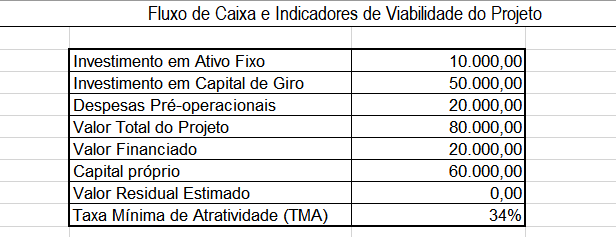
\includegraphics[width=13cm]{ws/w1.PNG}
    \caption{Fluxo de caixa e Indicadores de Viabilidade do Projeto.}
    \label{fig:www1}
\end{figure}
\FloatBarrier

\subsubsection{Ativo Fixo Operacional}

Para fins de início do projeto, tomando algumas facilitações técnicas com relação ao servidor e estruturação da parte de técnica da nossa empresa, a empresa pretende despender R\$ 10.000 para este fim.

\subsubsection{Ativo Fixo Administrativo}

Teremos gasto de R\$ 0 com este lado do projeto no início, qualquer outro profissional inserido à empresa, entrará nas despesas pré-operacionais.

\subsubsection{Despesas Pré-Operacionais}

A empresa pretende despender R\$ 20.000 para cobrir nossas despesas com pré-operação.

\subsubsection{Capital de Giro}

Para o capital de giro, manteremos R\$ 50.000.

\subsection{Fontes de Recursos}

Nossas fontes de recursos, no que tange a obtenção de material para o produto comercializado, são de custo zero; no que tange a obtenção de capital para o início das atividades da empresa, são de fontes privadas; no que tange a obtenção de mais capital futuro para outras operações, serão obtidas através de mercados financeiros descentralizados.

\subsection{Orçamentos}

Falaremos sobre nossos orçamentos para as seguintes áreas com base no financiamento planejado para o início de nossas atividades nas subseções a seguir.

\subsubsection{Orçamento da Área de Marketing}

40\% do nosso capital de giro será utilizado em marketing para promover a marca e nossos produtos: R\$ 20.000.

\subsubsection{Orçamento da Área Operacional}

20\% do nosso capital de giro será destinado à área operacional para fins de manter nossas qualidade e assegurar o funcionamento ideal de nossas práticas: R\$ 10.000.

\subsubsection{Orçamento da Área Administrativa}

40\% do nosso capital de giro ficará sobre posse da área administrativa para contornar eventuais necessidades: R\$ 40.000.

\subsection{Demonstração do Resultado do Exercício}

Sobre a nossa DRE, segue-se a imagem abaixo detalhando passo a passo.

\FloatBarrier
\begin{figure}[h]
    \centering
    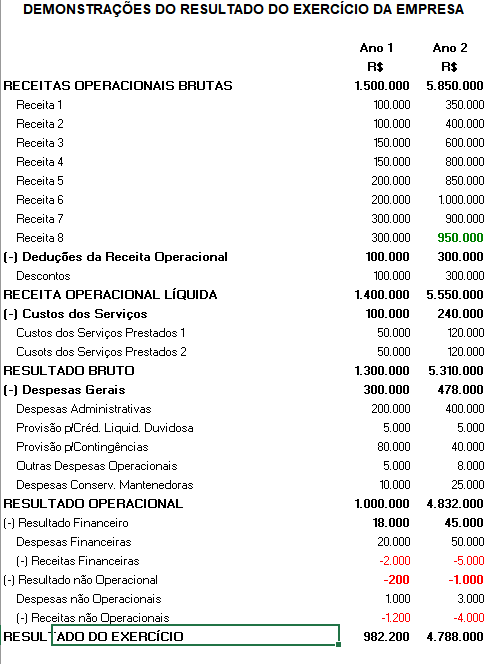
\includegraphics[width=13cm]{ws/w2.PNG}
    \caption{Demonstrações do Resultado do Exercício da {\it Diskify}.}
    \label{fig:www2}
\end{figure}
\FloatBarrier

\subsection{Fluxo de Caixa}

Faremos uma demonstração detalhada e gradual do avanço do fluxo de caixa da empresa.

\begin{itemize}

    \item Fluxo de Caixa Proveniente:
    \begin{itemize}
    
        \item Das Atividades Operacionais:
        \begin{itemize}
            \item (+) Recebimento de Clientes e outros: 5\%.
            \item (-) Pagamentos a Fornecedores: 0\%.
            \item (-) Pagamento a Funcionários: 0.1\%.
            \item (-) Recolhimento de Impostos: 0\%.
            \item (-) Pagamentos à Credores: 0\%.
            \item (=) Disponibilidades geradas pelas (aplicadas nas) atividades operacionais.
            \item ..
            \item Supondo um retorno mensal de R\$ 120.000 para início da empresa, temos que obteremos das atividades operacionais R\$ 117.600.
        \end{itemize}
        
        \item Das Atividades de Investimentos:
        \begin{itemize}
            \item (+) Recebimento de Venda de Imobilizado: 0\%.
            \item (-) Aquisição de Ativo Permanente: 0\%.
            \item (+) Recebimento de Dividendos: 5\%.
            \item (=) Disponibilidades geradas pelas (aplicadas nas) atividades de investimentos.
            \item ..
            \item Como nossa empresa se localiza e opera de forma remota, não há muitos gastos com infraestrutura críticos. Todos os nossos gastos são com isso são de alugueis e assinaturas e entram no capital de giro. Portanto, supondo os percentuais acima, podemos inferir que os dividendos das obras negociadas na nossa empresa geram R\$ 120.000: o mesmo que outras novas obras em desenvolvimento e produção na parte de operação da empresa.
        \end{itemize}
    
        \item Das Atividades de Financiamentos:
        \begin{itemize}
            \item (+) Novos Empréstimos: 0\%.
            \item (-) Amortização de Empréstimos: 0\%.
            \item (+) Emissão de Debêntures: 0\%.
            \item (+) Integralização de Capital: 5\%.
            \item (-) Pagamento de Dividendos: 5\%.
            \item (=) Disponibilidades geradas pelas (aplicadas nas) atividades de Financiamento
            \item ..
            \item Todo o capital gerado é automaticamente administrado pelo nosso contrato que distribui todas as atividades de financiamento aos respectivos destinatários; novas integrações de capital são feitas diretamente por terceiros, o que elimina qualquer custo ou necessidade de emissão de nossa parte. Portanto, tudo gerado aqui é utilizado para cobrir o fluxo dessa área.
        \end{itemize}
    
        \item AUMENTO/DIMINUIÇÃO NAS DISPONIBILIDADES
        \begin{itemize}
            \item DISPONIBILIDADES – no início do período
            \item DISPONIBILIDADES – no final do período
            \item ..
            \item Teremos menor capital em ativos gerando valor na rede para nosso contrato no início, mas com o tempo, o valor gerado - como visto acima - é incremental; ele é automaticamente adicionado ao capital de giro para possibilitar maior expansão do contrato na rede e adoção de subprojetos e capital de terceiros à nossa empresa.  
        \end{itemize}

    \end{itemize}

\end{itemize}

Para exemplificar o fluxo de caixa, utilizamos o seguinte planejamento com os índices de retorno do projeto.

\FloatBarrier
\begin{figure}[h]
    \centering
    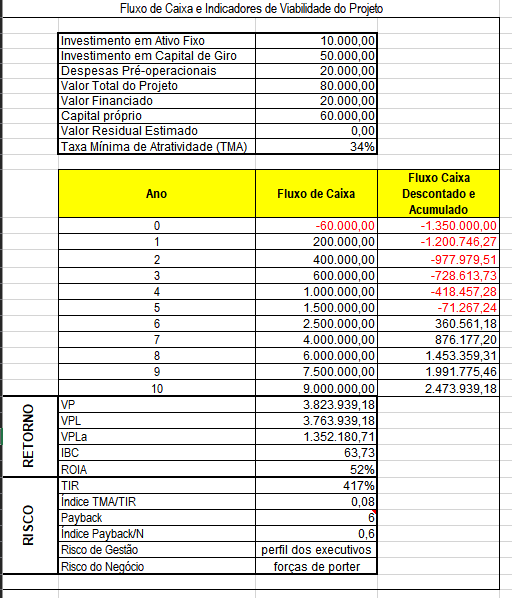
\includegraphics[width=13cm]{ws/w3.PNG}
    \caption{Fluxo de Caixa e Indicadores de Viabilidade do Projeto.}
    \label{fig:www3}
\end{figure}
\FloatBarrier

\subsection{Índices de Retorno e de Risco}

Definiremos os índices de retorno e risco nessa seção com base no que já foi dito e valores apresentados na última figura. Os indicadores são apresentados em percentuais e números absolutos com a finalidade de facilitar o entendimento da situação da empresa apresentada nos demonstrativos contábeis.

\subsubsection{Valor Presente}

Nosso valor presente é de R\$ 3.823.939,18 com base nos cálculos de fluxo de caixa.

\subsubsection{Valor Presente Líquido}

Nosso valor presente líquido é de R\$ 3.763.939,18 com base nos cálculos de fluxo de caixa.

\subsubsection{Valor Presente Líquido Anualizado}

Nosso valor presente líquido anualizado é de R\$ 1.352.180,71 com base nos cálculos de fluxo de caixa.

\subsubsection{Índice Benefício/Custo (IBC)}

Nosso índice benefício/custo (IBC) é 63,73 com base nos cálculos de fluxo de caixa.

\subsubsection{Retorno Adicional sobre Investimento (ROIA)}

Nosso retorno adicional sobre investimento (ROIA) é de 52\% com base nos cálculos de fluxo de caixa. 

\subsubsection{Taxa Interna de Retorno (TIR)}

Nossa taxa interna de retorno (TIR) é de 417\% com base nos cálculos de fluxo de caixa.

\subsubsection{PayBack}

Nosso PayBack ocorre no 6º período/ano com base nos cálculos de fluxo de caixa. 

\subsubsection{Índice TMA/TIR}

Nosso índice TMA/TIR é de 0,08 com base nos cálculos de fluxo de caixa.

\subsubsection{Índice PayBack/N}

Nosso índice de PayBack/N é de 0,6 com base nos cálculos de fluxo de caixa.

\subsubsection{Risco de Gestão}

O Risco de Gestão, que está associado ao grau de competência do grupo gestor em empreendimentos similares, à competência técnica em produção e comercialização (incluindo-se aí a motivação para a inovação) e à saúde financeira do grupo em análise. Sobre esses aspectos, nosso grupo é o mais competente para o objetivo da empresa devido à nossa facilidade de obtenção de profissionais altamente dentro do ambiente a que se insere a proposta, e está familiarizado com empreendimentos parecidos devido à natureza do nosso setor também; quanto a comercialização, ela deve ser automatizada e procedural - altamente familiar a outros tipos de negociações corriqueiras: o que a torna muito intuitiva e, portanto, de boa qualidade; quanto a produção, pode se dizer que ela é facilmente realizada por nossos fornecedores e é de praxe, logo não há nada de diferente nela que pressuponha um maior risco do que o original. A motivação para tal tarefa se dá justamente pela imersão dos colaboradores no ambiente e a capacidade de fazer mais capital para si e uma causa em comum que os beneficiará direta e indiretamente; sobre a saúde financeira, todos que participam precisam estar bem para que possam primeiramente estarem atuando, caso contrário, não teriam nem mesmo acesso as funcionalidades mais abstratas da aplicação para desenvolver melhorias à empresa - logo, não é um risco a nós. Consideramos que o risco de gestão é baixo ou praticamente inexistente.

\subsubsection{Risco do Negócio}

O Risco de Negócio, que está associado a fatores conjunturais e não controláveis que afetam o ambiente do projeto. Inclui-se aí o grau de concorrência, as barreiras a novos entrantes, as tendências da economia e do setor em análise. Pode-se utilizar os conceitos das 5 Forças de Porter (análise competitiva da indústria) para identificar o risco do negócio. Sobre o grau de concorrência, com base no que obtemos com a análise das Forças de Porter, a média geral do setor é de 2,39 - o que explicita um ambiente de intensidade competitiva média -; também, descrevemos que as barreiras a novos entrantes são basicamente nulas devidas a maior parte dos códigos na web 3.0 serem open-source, contudo, há o custo inicial de publicar contratos na rede - por isso se faz necessário o capital de investimento em ativo fixo aqui; as tendências do setor em análise são de um aumento em 5 anos do mercado como um todo e um aumento de público-usuário das tecnologias, com um maior conhecimento sobre este mercado do público mediano e fora dele, logo, a economia desta área é saudável e tende a prosperar. O posicionamento estratégico global (PEG) da empresa é favorável segundo a análise de ambiente externo e interno; portanto, o risco de negócio é médio.

\subsection{Análise de Viabilidade Financeira e de Risco}

A nossa análise de viabilidade financeira e de risco demonstrou que temos uma visão estrutural e organizacional de políticas de desenvolvimento, de comércio e financeiras muito clara e aberta a terceiros investidores - que se atraem não somente pelo custo oportunidade e nossa ROIA, mas, também, a possibilidade de avaliar nosso estado na rede e ponderar a sua exposição ao risco durante o desenvolvimento, comprando ou vendendo seus tokens de governança com outros especuladores, ou simplesmente investindo nos ativos da empresa ou, até mesmo, ajudando na divulgação para benefício próprio e, por conseguinte, a nossa marca. Fizemos um investimento modesto para iniciar as atividades da empresa porque temos facilidade na obtenção dos nossos recursos, nossas fontes participam com seus custos no processo de evolução dos seus ativos por nós - o que faz que nossos orçamentos também sejam razoáveis. A demonstração do resultado do exercício (DRE) da empresa mostrou que a nossa conduta é saudável e lucrativa, pois nosso fluxo de caixa nos facilita em estruturar a transparência da empresa em suas atividades financeiras de forma que fica fácil a compreensão dos envolvidos e, por conseguinte, possibilita o aporte de capital de terceiros em momentos de oportunidade conforme estes a notem: mantendo, assim, uma postura altamente competitiva no mercado com consistência. Nossos índices de retorno e de risco apontam para um cenário muito atrativo, a taxa de retorno sobre investimento e o valor presente líquido demonstram uma empresa flexível com alta capacidade de adaptação a novas oportunidades, mas também de integração e acúmulo gradual de capital ativo na plataforma - que nos paga constantemente por meio de dividendos inteligentes (mecanismo desenvolvido por nós para facilitar e dar veracidade aos valores criados na rede). Portanto, a análise relata que devemos proceder com a implementação e dar início as atividades mercadológicas da {\it Diskify}.

\section{Adicionais}

Alguns adicionais sobre o projeto e informações relevantes para o entendimento da filosofia da DAO e suas motivações enquanto comunidade.

\subsection{Elicitando as referências}

Conhecimentos sobre o mercado financeiro sobre preços dos cripto-ativos e sobre fatos históricos relacionados podem ser encontrados em: \cite{rrf1}\cite{rrf12}\cite{rrf8}\cite{rrf11}\cite{rrf4}. Conhecimentos sobre a tecnologia por trás das NFTs: \cite{rrf5}
\cite{rrf9}\cite{rrf7}. Conhecimentos sobre o mundo DeFi: \cite{rrf3}\cite{rrf6}. Curiosidades sobre o artista Beeple e sua obra mais valiosa: \cite{rrf2}.

\subsection{Link para Vídeo sobre a Implementação do Projeto}

Este link é para o vídeo da implementação das fundações da aplicação desenvolvida e sua lógica de funcionamento, explicando cada item do código e sua relevância na automatização dos contratos: https://youtu.be/UnzlorkFw9g.

\newpage
\printbibliography  

\end{document}
